\chapter{Unrestringierte Optimierung}
\label{ch:optimierung}

Optimierung ist ein omnipräsentes Phänomen, dass nicht nur in der abstrakten Welt der Mathematik existiert. Viel mehr stellt es ein naturgegebenes Prinzip dar, welches überall um uns herum zur Anwendung kommt. 
In der Physik beispielsweise spielt Optimierung eine wesentliche Rolle bei der Modellierung von Energiezuständen auf unterschiedlichen Skalen: 
Moleküle formieren sich in einer Art, die die Gesamtenergie des Teilchensystems unter Berücksichtigung aller wechselseitigen Kräfte minimiert. 
Gleichzeitig strebt das Universum mit all seinen Planeten, Sternen und Galaxien nach einem Zustand von maximaler Verteilung, beschrieben durch die thermodynamische Größe der Entropie. 
Auch hier folgt die Zunahme der Entropie dem Prinzip der Energieminimierung des Gesamtsystems.
Menschen betreiben seit jeher Optimierung in den verschiedensten Anwendungen, oft mit unterschiedlichen Motivationen. 
Flugzeuge werden von Ingenieuren so entworfen und gebaut, dass sie möglichst stromlinienförmig aussehen, um damit den Reibungswiderstand in der Luft zu minimieren und gleichzeitig den nötigen Auftrieb für einen sicheren Flug zu erzeugen. 
Fondmanager streben danach Portfolios zu erstellen, deren Gewinn möglichst maximal ist und dennoch Spekulationsrisiken vermeiden. 
Die gesamte Automatisierung der Industrie, angefangen bei den ersten Manufakturen hin zu modernen vollautomatischen Roboterfabriken, dient lediglich dem Prinzip der Gewinnmaximierung durch Minimierung der Produktionskosten.

Es ist also nicht wirklich überraschend, dass sich ein gesamtes Teilgebiet der Angewandten Mathematik mit der Theorie der Optimierung befasst und somit dazu beiträgt viele Optimierungsprobleme besser zu verstehen und zu lösen, seien es Probleme des Alltags oder grundlegende Gesetzmäßigkeiten bei der Ergründung des Kosmos. 
Im folgenden Abschnitt wollen wir uns speziell mit der unbeschränkten (oder: unrestringierten) Optimierung beschäftigen und uns nützliche Werkzeuge zum Lösen von numerischen Problemstellungen herleiten. 
Nach einer allgemeinen mathematischen Einführung in Kapitel \ref{s:opt_grundlagen} beginnen wir in Kapitel \ref{s:abstiegsverfahren} mit einer Klasse von Algorithmen, die einer einfachen Idee folgen: die Abstiegsverfahren.
In Kapitel 
%\ref{s:cg_verfahren} 
2.2 
behandeln wir insbesondere das Verfahren der konjugierten Gradienten, welches zur iterativen Lösung von großen, linearen Gleichungssystemen mit besonderen Eigenschaften genutzt werden kann. 
Zum Schluss untersuchen wir in Kapitel 
2.3
%\ref{s:primal-dual} 
einen modernen primal-dualen Optimierungsalgorithmus zur Lösung von konvexen, nicht-glatten Problemen.

\section{Mathematische Grundlagen}
\label{s:opt_grundlagen}
Im Folgenden wollen wir die mathematischen Grundlagen zur Untersuchung von allgemeinen Optimierungsproblemen einführen. 
Wir folgen hierbei zu großen Teilen der Notation von Nocedal und Wright \cite{nocedal_1999}. 
Wir beginnen mit der Definition des allgemeinen Optimierungsproblems, welches wir im Verlauf der Vorlesung nur für Spezialfälle näher untersuchen werden.
\begin{definition}{Allgemeines Optimierungsproblem}{}
Sei $\Omega \subset \mathbb{R}^n$ ein offenes, zusammenhängendes Gebiet und sei $F \colon \Omega \rightarrow \mathbb{R}$ eine reellwertige Funktion, welche wir \emph{Zielfunktion} nennen. Unser Ziel ist es einen unbekannten Vektor $x \in \Omega$, auch Parametervektor genannt, zu finden, welcher das folgende allgemeine Optimierungsproblem löst.
\begin{equation}
\label{eq:optimierungsproblem_allgemein}
\min_{x \in \Omega} F(x) \qquad \text{ mit } 
\begin{cases}
c_i(x) \ = \ 0, \quad &i \in \mathcal{E},\\
c_i(x) \ \geq \ 0, \quad &i \in \mathcal{I}.
\end{cases}
\end{equation}
Die reellwertigen Funktionen $c_i \colon \Omega \rightarrow \mathbb{R}$ bilden einen Vektor von \emph{Nebenbedingungen}, welcher das Optimierungsproblem restringiert. Die Indexmengen $\mathcal{E}$ und $\mathcal{I}$ legen hierbei fest, ob es ich bei der jeweiligen Nebenbedingung um eine Gleichung oder eine Ungleichung handelt.
\end{definition}
Zur Veranschaulichung betrachten wir ein zweidimensionales Beispiel für ein beschränktes, nichtlineares Optimierungsproblem.
\begin{example}{}{}
Betrachte das mathematische Problem:
\begin{equation*}
\min_{x \in \mathbb{R}^2} (x_1 - 2)^2 + (x_2 - 1)^2
\end{equation*}
unter den Nebenbedingungen $x_1^2 - x_2 \leq 0$ und $x_1 + x_2 \leq 2$. Wir können dieses Problem in die allgemeine Form des Optimierungsproblems \eqref{eq:optimierungsproblem_allgemein} umschreiben als:
\begin{equation*}
\min_{x \in \mathbb{R}^2} F(x) \ = \ \min_{x \in \mathbb{R}^2} (x_1 - 2)^2 + (x_2 - 1)^2, \qquad \text{ mit }
\begin{cases}
c_1(x) = -x_1^2 + x_2 \geq 0,\\
c_2(x) = -x_1 - x_2 + 2 \geq 0.
\end{cases}
\end{equation*}
Hierbei gilt für die Indexmengen $\mathcal{I} = \lbrace 1,2 \rbrace$ und $\mathcal{E} = \emptyset$.
Visualisiert man die Niveaulinien der Zielfunktion $F$ zusammen mit den Nebenbedingungen, so sieht man, dass das globale Minimum der quadratischen Funktion $F$, nämlich $x = (x_1, x_2)^T = (2,1)^T$, nicht in der erlaubten Menge der Parameter liegt, welche durch die Nebenbedingungen beschrieben ist. Trotzdem existiert ein eindeutiges globales Minimum des beschränkten Optimierungsproblems, nämlich $x = (x_1, x_2)^T = (x,y)^T$.
\end{example}
Im Rahmen dieser Vorlesung wollen wir uns auf eine bestimmte Klasse von allgemeinen Optimierungsproblemen konzentrieren, den \textit{unbeschränkten} oder \textit{unrestringierten} Optimierungsproblemen.
\begin{definition}{Unbeschränkte Optimierung}{}
Liegt ein allgemeines Optimierungsproblem der Form \eqref{eq:optimierungsproblem_allgemein} ohne Nebenbedingungen vor, d.h., für die Indexmengen gilt $\mathcal{E} = \mathcal{I} = \emptyset$, so sprechen wir von einem \emph{unbeschränkten} oder \emph{unrestringierten Optimierungsproblem}.
\end{definition}
\begin{remark}{}{}
Häufig lassen sich restringierte Optimierungsprobleme in unrestringierte Optimierungsprobleme überführen, indem man zusätzliche Strafterme zur Zielfunktion hinzufügt, die eine Verletzung der ursprünglichen Nebenbedingungen zwar mit Kosten belegt, diese jedoch grundsätzlich erlaubt. Hierbei spricht man auch von \textit{relaxierten Optimierungsproblemen}.
\end{remark}
Neben der Unterscheidung von Optimierungsproblemen in beschränkte und unbeschränkte Formulierungen, lassen sich noch weitere Kriterien zur Charakterisierung eines Optimierungsproblems heran ziehen:
\begin{itemize}
\item \textbf{Anzahl der unbekannten Parameter}, z.B. groß oder klein
\item \textbf{Eigenschaften der Zielfunktion}, z.B. Linearität, Konvexität, Differenzierbarkeit
\item \textbf{Charakteristik des Optimums}, z.B. Sattelpunkt, lokales oder globales Optimum
\item \textbf{Modelleigenschaften}, z.B. stochastisch oder deterministisch
\end{itemize}
Für den weiteren Verlauf der Vorlesung gehen wir immer, wenn nicht anders beschrieben, von einem unrestringierten Optimierungsproblem aus.
Da wir uns intensiv mit der Bestimmung und numerischen Approximation von Optima beschäftigen werden, macht es Sinn diese zuerst formal zu beschreiben.
\begin{definition}{Stationärer Punkt}{}
Sei $\Omega \subset \mathbb{R}^n$ ein offenes, zusammenhängendes Gebiet und sei $F \colon \Omega \rightarrow \mathbb{R}$ eine reellwertige Funktion. 
Wir nennen einen Punkt $x^* \in \Omega$ \emph{stationären Punkt} von $F$, falls er die Bedingung $\nabla F(x^*) = 0$ erfüllt.
\end{definition}
\begin{definition}{Lokales und globales Minimum}{}
Sei $\Omega \subset \mathbb{R}^n$ ein offenes, zusammenhängendes Gebiet und sei $F \colon \Omega \rightarrow \mathbb{R}$ eine reellwertige Funktion. 
Wir nennen einen Punkt $x^* \in \Omega$ ein \emph{lokales Minimum} der Funktion $F$, falls es eine lokale Umgebung $U \subset \Omega$ von $x^* \in U$ gibt, so dass für alle $x \in U$ gilt:
\begin{equation}
\label{eq:lokales_minimum}
F(x^*) \leq F(x), \quad \forall x \in U.
\end{equation}
Wir nennen $x^* \in \Omega$ ein \emph{globales Minimum} von $F$, falls die Ungleichung \eqref{eq:lokales_minimum} für jede beliebige Umgebung $U \subset \Omega$ gilt und somit insbesondere für $U = \Omega$. 
\end{definition}
\begin{remark}{}{}
In obiger Definition sprechen wir nur von Minima, jedoch ist klar, dass sich jedes Maximierungsproblem durch einen Vorzeichenwechsel leicht in ein Minimierungsproblem umschreiben lässt, d.h.,
\begin{equation*}
\max_{x\in\Omega} F(x) \ \Leftrightarrow \ \min_{x\in\Omega} -F(x) \ := \ \min_{x_\in\Omega} G(x).
\end{equation*}
\end{remark}
Da wir nun eine Bedingung für das Vorliegen eines lokalen Minimums haben, können wir mit folgenden Satz die notwendigen Bedingungen für solch ein lokales Minimum angeben.
\begin{theorem}{Notwendige Optimalitätsbedingungen erster Ordnung}{}
\label{thm:minimum_notwendig}
Sei $\Omega \subset \mathbb{R}^n$ ein offenes, zusammenhängendes Gebiet und sei $F \colon \Omega \rightarrow \mathbb{R}$ eine reellwertige Funktion. 
Sei $x^*\in \Omega$ ein lokales Minimum von $F$ in $\Omega$ und die Funktion $F$ sei stetig differenzierbar in einer lokalen, offenen Umgebung $U \subset \Omega$ von $x^*$. 
Dann gilt $\nabla F(x^*) = 0$.
\end{theorem}
\begin{proof}
Wir führen einen Beweis durch Widerspruch. 
Nehmen wir also an, dass $x^* \in \mathbb{R}$ ein lokales Minimum von $F$ sei, jedoch aber $\nabla F(x^*) \neq 0$ gelte.
Wir wählen den Richtungsvektor $\vec{p} \coloneqq -\nabla F(x^*) \neq 0$. 
Es ist somit klar, dass 
\begin{equation*}
\langle \vec{p}, \nabla F(x^*) \rangle \ = \ - \langle \nabla F(x^*), \nabla F(x^*) \rangle \ = \ - ||\nabla F(x^*)||^2 \ < \ 0.
\end{equation*}
Da $\nabla F$ nach Vorraussetzung stetig in einer lokalen Umgebung $U \subset \Omega$ von $x^*$ ist existiert ein $T > 0$, so dass auch gilt:
\begin{equation*}
\langle \vec{p}, \nabla F(x^* + t\vec{p}) \rangle < 0, \quad \text{ für alle } t\in [0,T].
\end{equation*}
Nach dem Satz von Taylor gilt aber auch für jedes $t \in [0,T]$:
\begin{equation*}
F(x^* + t\vec{p}) \ = \ F(x^*) +~\underbrace{t\langle \vec{p}, \nabla F(x^* + t\vec{p}) \rangle}_{<~0}, \quad \text{ für ein } \tilde{t} \in (0,t).
\end{equation*}
Somit gilt also $F(x^* + t\vec{p}) < F(x^*)$ und wir haben offenbar eine Richtung $\vec{p} \in \mathbb{R}^n / \lbrace 0\rbrace$ gefunden in der die Funktionswerte von $F$ abnehmen. 
Also ist $x^* \in \Omega$ kein lokales Minimum von $F$. 
Das ist aber ein Widerspruch zur Annahme und somit ist die Behauptung bewiesen.
\end{proof}
\begin{corollary}{}{}
Jedes lokale Minimum $x^* \in \Omega$ einer Funktion $F \colon \Omega \rightarrow \mathbb{R}$ ist ein stationärer Punkt.
\end{corollary}
\begin{remark}{}{}
Die Umkehrung der Aussage in Satz \ref{thm:minimum_notwendig} gilt im Allgemeinen nicht. 
Man betrachte zum Beispiel die Funktion $F(x) \coloneqq -x^3$. 
Diese besitzt einen stationären Punkt in $x^* = 0$, d.h., es gilt $\nabla F(0) = 0$. 
Dennoch handelt es sich hierbei nicht um ein lokales Optimum, sondern lediglich um einen Sattelpunkt. 
Aus diesem Grund handelt es sich nur um notwendige Bedingungen.
\end{remark}
Bei der Suche nach lokalen Minima einer Funktion $F$ lässt sich ein weiteres Kriterium anwenden, welches die zweite Ableitung der Funktion verwendet.
\begin{theorem}{Notwendige Optimalitätsbedingungen zweiter Ordnung}{}
Sei $\Omega \subset \mathbb{R}^n$ ein offenes, zusammenhängendes Gebiet und sei $F \colon \Omega \rightarrow \mathbb{R}$ eine reellwertige Funktion. 
Sei $x^*\in \Omega$ ein lokales Minimum von $F$ in $\Omega$ und die Hessematrix $\nabla^2 F$ von $F$ sei stetig in einer offenen Umgebung $U \subset \Omega$ von $x^*$. 
Dann gilt $\nabla F(x^*) = 0$ und $\nabla^2 F(x^*)$ ist positiv semidefinit, d.h., es gilt $\langle \vec{p}, \nabla^2F(x^*) \vec{p} \rangle \geq 0$ für alle $\vec{p} \in \mathbb{R}^n$.
\end{theorem}
\begin{proof}[Beweis:]
Der erste Teil der Behauptung folgt bereits aus Satz \ref{thm:minimum_notwendig}, so dass wir uns nur auf den Beweis für die zweite Behauptung konzentrieren müssen. 
Wir führen wieder einen Beweis durch Widerspruch. 
Sei $x^* \in \Omega$ nach Vorraussetzung ein lokaler Minimierer von $F$, das heißt nach Satz \ref{thm:minimum_notwendig} gilt $\nabla F(x^*) = 0$. 
Wir nehmen an, dass $\nabla^2 F(x^*)$ nicht positiv semidefinit ist. 
Dann können wir einen Vektor $\vec{p} \in \mathbb{R}^n / \lbrace 0\rbrace$ finden, so dass
\begin{equation*}
\langle \vec{p}, \nabla^2F(x^*)\vec{p} \rangle \ < \ 0
\end{equation*}
gilt. 
Da $\nabla^2 F$ nach Vorraussetzung stetig ist in einer lokalen Umgebung $U \subset \Omega$ von $x^*$ existiert ein $T > 0$, so dass
\begin{equation*}
\langle \vec{p}, \nabla^2F(x^* + t\vec{p})\vec{p} \rangle \ = \ 0, \quad \text{ für alle } t\in[0,T]. 
\end{equation*}
Nach dem Satz von Taylor gilt jedoch für alle $t \in (0,T)$
\begin{equation*}
F(x^* + t\vec{p}) \ = \ F(x^*) +~\underbrace{t\langle \vec{p}, \nabla F(x^* + t\vec{p}) \rangle}_{=~0} \, + \, \frac{1}{2}t^2\underbrace{\langle \vec{p}, \nabla^2 F(x^* + \tilde{t}\vec{p})\vec{p}\rangle}_{<~0}, \quad \text{ für ein } \tilde{t} \in (0,t).
\end{equation*}
Damit folgt also, dass $F(x^* + t\vec{p}) < F(x^*)$ gilt. Wir haben also eine Richtung $\vec{p} \in \mathbb{R}^n/\lbrace 0 \rbrace$ gefunden entlang der die Funktionswerte von $F$ abnehmen. 
Damit folgt, dass $x^*$ kein lokales Minimum von $F$ ist, was aber im Widerspruch zur Annahme steht. 
Das beweist die Aussage des Satzes.
\end{proof}
Schlussendlich wollen wir auch eine hinreichende Bedingung für das vorliegen eines lokalen Minimums angeben.
\begin{theorem}{Hinreichende Optimalitätsbedingungen zweiter Ordnung}{minimum_hinreichend}
Sei $\Omega \subset \mathbb{R}^n$ ein offenes, zusammenhängendes Gebiet und sei $F \colon \Omega \rightarrow \mathbb{R}$ eine reellwertige Funktion. 
Sei $x^*\in \Omega$ ein lokales Minimum von $F$ in $\Omega$ und die Hessematrix $\nabla^2 F$ von $F$ sei stetig in einer offenen Umgebung $U \subset \Omega$ von $x^*$. 
Außerdem gelte
\begin{enumerate}[label=(\roman*)]
\item $\nabla F(x^*) \ = \ 0$,
\item $\nabla^2 F(x^*)$ ist positiv definit.
\end{enumerate}
Dann ist $x^* \in \Omega$ ein striktes lokales Minimum von $F$.
\end{theorem}
\begin{proof}
Da die Hessematrix $\nabla^2 F$ von $F$ stetig und positiv definit in $x^* \in \Omega$ ist nach Vorraussetzung können wir einen Radius $r > 0$ finden, so dass $\nabla^2 F(x)$ positiv definit ist für alle $x \in B_r(x^*)$. 
Für jeden Vektor $\vec{p} \in \mathbb{R}^n / \lbrace 0\rbrace$ mit $||\vec{p}|| < r$ gilt dann nach dem Satz von Taylor:
\begin{equation*}
F(x^* + \vec{p}) \ = \ F(x^*) +~\underbrace{\langle \vec{p}, \nabla F(x^*) \rangle}_{=~0} + \frac{1}{2} \langle \vec{p}, \nabla^2F(x^* + t\vec{p})\vec{p} \rangle, \quad \text{ für ein } t\in (0,1).
\end{equation*}
Da $||t\vec{p}|| < r$ ist nach Konstruktion wissen wir, dass
\begin{equation*}
\langle \vec{p}, \nabla^2F(x^* + t\vec{p})\vec{p} \rangle \ > \ 0
\end{equation*}
gilt und somit schon $F(x^* + \vec{p}) > F(x^*)$ gelten muss. 
Da $\vec{p} \in \mathbb{R}^n / \lbrace 0 \rbrace$ mit $||\vec{p}|| < r$ beliebig gewählt war handelt es sich bei $x^* \in \Omega$ um ein striktes lokales Minimum der Funktion $F$.
\end{proof}
\begin{remark}{}{}
Die in Satz \ref{thm:minimum_hinreichend} genannten Bedingungen sind nur hinreichend, jedoch nicht notwendig für das Vorliegen eines strikten lokalen Minimums. 
Dies sieht man ein, wenn man beispielsweise die Funktion $F(x) \coloneqq x^4$ betrachtet. $F$ besitzt ein striktes lokales Minimum in $x=0$ und es gilt $\nabla F(0) = 0$, jedoch verschwindet die zweite Ableitung $\nabla^2F(0) = 0$ und ist somit nicht positiv definit.
\end{remark}
Eine äußerst wertvolle Eigenschaft bei der Optimierung ist die Konvexität einer Zielfunktion, da jedes lokale Optimum einer konvexen Funktion bereits ein globales Optimum ist.
\begin{definition}{Konvexität}{}
Sei $\Omega \subset \mathbb{R}^n$ ein offenes, zusammenhängendes Gebiet und sei $F \colon \Omega \rightarrow \mathbb{R}$ eine reellwertige Funktion. Wir nennen $F$ \emph{konvex} wenn für beliebige Vektoren $x,y \in \Omega$ die folgende Ungleichung für alle $0 \leq \alpha \leq 1$ gilt:
\begin{equation*}
F(\alpha x + (1-\alpha)y) \ \leq \ \alpha F(x) + (1-\alpha)F(y).
\end{equation*}
Anschaulich bedeutet Konvexität einer Funktion $F$, dass jede Verbindungsgerade zwischen zwei Punkten $x,y \in \Omega$ oberhalb des Graphen der Funktion $F$ durch die Punkte $x$ und $y$ verläuft.
\end{definition}

\section{Abstiegsverfahren}
\label{s:abstiegsverfahren}
Zu Anfang dieser Vorlesung möchten wir eine Klasse von Algorithmen zur Optimierung von Funktionen besprechen, die einer simplen und anschaulichen Idee folgen: die sogenannten \textit{Abstiegsverfahren} oder auch \textit{Liniensuchverfahren} (im Englischen: \textit{line search methods}).
Diese wurden bereits kurz im Zusammenhang mit dem Gauss-Newton Verfahren in der Vorlesung \glqq Einführung in die Numerik\grqq~in \cite[Kapitel 5.4]{numerik1} erwähnt, jedoch nicht ausführlich diskutiert. 
Dies wollen wir im Folgenden nachholen.

Sei im Folgenden $\Omega \subset \mathbb{R}^n$ ein offenes, zusammenhängendes Gebiet und sei $F \colon \Omega \rightarrow \mathbb{R}$ eine differenzierbare, reellwertige Funktion, die es in dem Gebiet zu minimieren gilt.
Die allgemeine Idee der Abstiegsverfahren ist es nun ausgehend von einem aktuellen Punkt $x_k \in \Omega$ einen Schritt in eine Richtung $\vec{p}_k \in \mathbb{R}^n$ zu machen, so dass der Funktionswert von $F$ in dem neuen Punkt $x_{k+1}$ abnimmt.
Das bedeutet wir versuchen ein Iterationsschema der Form
\begin{equation}
\label{eq:abstiegsverfahren}
x_{k+1} \ = \ x_k + \alpha_k \vec{p}_k, \quad \alpha_k > 0,
\end{equation}
zu konstruieren, das in jedem Schritt den Funktionswert $F(x_k)$ verringert bis keine Verbesserung mehr möglich ist.
Die Schrittweite $\alpha_k > 0$ in Richtung $\vec{p}_k \in \mathbb{R}^n$ wird hierbei auch in jedem Schritt des Abstiegsverfahrens gewählt.

\subsection{Gradientenabstiegsverfahren}
\label{ss:gradient_descent}
Zuerst beschäftigen wir uns mit dem wohl bekanntesten Abstiegsverfahren, dem \textit{Gradientenabstiegsverfahren} (im Englischen: \textit{gradient descent}). 
Dieses wird wegen seiner Einfachheit für viele numerische Optimierungsprobleme verwendet. 

Da $F$ differenzierbar ist können wir dessen Gradienten in jedem Punkt $x \in \Omega$ betrachten. 
Der Gradient $\nabla F(x)$ beschreibt bekanntlich eine Richtung des stärksten Anstiegs der Funktion $F$ im Punkt $x$ und dementsprechend zeigt der negative Gradient $-\nabla F(x)$ in die Richtung des stärksten Abstiegs.
Das lässt sich auch formal zeigen indem wir uns die Taylorapproximation erster Ordnung der Funktion $F$ in allgemeine Richtung $\vec{p}$ mit Schrittweitenlänge $\alpha > 0$ für den $k$-ten Schritt des Abstiegsverfahren näher anschauen.
\begin{equation*}
F(x_k + \alpha \vec{p}) \ = \ F(x_k) + \alpha \langle \nabla F(x_k), \vec{p} \rangle + \mathcal{O}(\mathcal{H}[F(x_k)]),
\end{equation*}
wobei $\mathcal{H}[F]$ die Hesse-Matrix der Funktion $F$ bezeichnet.
Es wird also klar, dass die Änderung der Funktionswerte von $F$ im Wesentlichen von der Größe des Terms $\langle \nabla F(x_k), \vec{p} \rangle$ bestimmt wird.
Wir können also für eine maximale Verringerung der Funktion $F$ nach derjenigen Richtung mit Einheitslänge suchen, die das folgende Minimierungsproblem löst:
\begin{equation}
\label{eq:optimization_direction}
\min_{\vec{p} \in \mathbb{R}^n} \langle \nabla F(x_k), \vec{p} \rangle, \quad \text{ mit } ||\vec{p}|| = 1. 
\end{equation}
Da außerdem
\begin{equation*}
 \langle \nabla F(x_k), \vec{p} \rangle \ = \ ||\nabla F(x_k)||~||\vec{p}|| \cos(\theta) 
\end{equation*}
gilt, wobei $\theta$ der Winkel zwischen den Vektoren $\nabla F(x_k)$ und $\vec{p}$ bildet, können wir das Problem \eqref{eq:optimization_direction} umschreiben zu
\begin{equation*}
\min_{\theta \in [0,2\pi)} ||\nabla F(x_k)|| \cos(\theta).
\end{equation*}
Der Kosinus nimmt sein Minimum von $\cos(\theta)=-1$ in $\theta = \pi$ an und damit erhalten wir, dass die optimale Richtung $\vec{p} \in \mathbb{R}^n$ folgenden Zusammenhang erfüllen muss:
\begin{equation*}
\langle \vec{p}, \frac{\nabla F(x_k)}{||\nabla F(x_k)||}\rangle \ = \ -1.
\end{equation*}
Daraus folgt aber auch schon, dass
\begin{equation}
\label{eq:optimal_direction}
\vec{p} \ = \ -\frac{\nabla F(x_k)}{||\nabla F(x_k)||}.
\end{equation}
Das bedeutet, dass der Funktionswert von $F$ am meisten in Richtung des negativen Gradienten abnimmt.

Da wir daran interessiert sind die Funktion $F$ schnellstmöglich zu minimieren, macht es Sinn in dieser Richtung nach einem lokalen Minimum zu suchen. 
Aus dieser Idee heraus lässt sich bereits ein sehr simpler Algorithmus zur Minimierung von $F$ formulieren. Sei $x_0 \in \Omega$ ein beliebiger Startwert, dann können wir iterativ eine Folge von Punkten $x_1,\ldots$ bestimmen, deren Funktionswerte monoton fallen sollten: 
\begin{equation}
\label{eq:gradient_descent_simple}
x_{k+1} \ = \ x_k - \nabla F(x_k).
\end{equation}
Intuitiv stoppt man das Iterationsschema \eqref{eq:gradient_descent_simple} sobald die Folge der Funktionswerte $F(x_k)$ nicht mehr kleiner wird.
Man sieht leicht ein, dass das simple Iterationsschema \eqref{eq:gradient_descent_simple} ein Spezialfall des allgemeinen Abstiegsverfahrens \eqref{eq:abstiegsverfahren} mit fester Schrittweite $\alpha_k = ||\nabla F(x_k)||$ und Richtung $\vec{p}_k = \nabla F(x_k)$ ist.
Diese einfache Methode lässt sich durch folgenden Algorithmus implementieren.

\begin{algorithm}{Simples Gradientenabstiegsverfahren}{}
\label{alg:gradient_descent_simple}
\begin{algorithmic}
\STATE \textbf{function} $[x^*, F(x^*)]= $\texttt{gradientDescentSimple}$(F,\nabla F, x_0)$ \{
%\STATE ~
\STATE \# Initialisierung
\STATE $x_k = x_0$
\STATE $F(x_{k+1}) = -$\texttt{Inf}
\STATE ~
\WHILE{$F(x_{k+1}) - F(x_k) < 0$}
%\STATE ~
\STATE \# Update in Richtung des größten Gradientenabstiegs
\STATE $x_{k+1} = x_k - \nabla F(x_k)$
%\STATE ~
\ENDWHILE
\STATE ~
\STATE \# Ausgabe des letzten Punktes
\STATE $x^* = x_k$
\STATE $F(x^*) = F(x_k)$
\STATE \}
\end{algorithmic}
\end{algorithm}
Unglücklicherweise ist Algorithmus \ref{alg:gradient_descent_simple} in dieser Form praktisch nicht anwendbar. Warum dies so ist sieht man leicht an folgenden Beispiel.
\begin{example}{}{}
\label{ex:gradient_descent_simple}
Sei $\Omega = \mathbb{R}$ und sei $F(x) \coloneqq |x|$. 
Man beachte, dass $F$ überall differenzierbar ist, außer an der Stelle $x=0$. Das eindeutig bestimmte, globale Minimum der konvexen, nichtlinearen Funktion $F$ wird ebenfalls in $x^* = 0$ angenommen. 
Definiert man $\nabla F(0) \coloneqq 0$ in der Singularität, so erhält man das Minimum $x^* = 0$ durch Algorithmus \ref{alg:gradient_descent_simple} nur für Startwerte $x_0 \in \mathbb{Z}$. 
Wähle zum Beispiel den Startwert $x_0 = 0.5$, so terminiert das Gradientenabstiegsverfahren bereits nach dem ersten Schritt ohne eine gute Näherung an $x^* = 0$ zu liefern.
\end{example}
Wie das Beispiel \ref{ex:gradient_descent_simple} zeigt, besteht bei dem Gradientenabstiegsverfahren in Algorithmus \ref{alg:gradient_descent_simple} die Gefahr das Minimum zu überspringen. 
Aus diesem Grund kommt man auf die Idee die Schrittweitengröße $\alpha_k > 0$ in \eqref{eq:abstiegsverfahren} genügend klein zu wählen.
Damit diese feste Schrittweite unabhängig von der Magnitude des Gradienten $\nabla F$ ist, normiert man in der Regel die Richtung des steilsten Gradientenabstiegs durch die Norm des Gradienten, d.h., wir erhalten eine steuerbare Version des Gradientenabstiegsverfahrens in \eqref{eq:gradient_descent_simple} durch:
\begin{equation}
\label{eq:gradient_descent_control}
x_{k+1} \ = \ x_k - \tau \frac{\nabla F(x_k)}{||\nabla F(x_k)||}, \quad \tau > 0 .
\end{equation}
Das Iterationsschema \eqref{eq:gradient_descent_adaptive} ist wiederum ein Spezialfall des allgemeinen Abstiegsverfahrens in \eqref{eq:abstiegsverfahren} für eine feste Schritteweite $\alpha_k = \tau > 0$ und Richtung $\vec{p}_k = -\nabla F(x_k) / ||\nabla F(x_k)||$.
Es ist klar, dass durch eine kleinere Schrittweite $\tau > 0$ das lokale Minimum der Funktion $F$ im Punkt $x^* \in \Omega$ immer besser angenähert werden kann. 
Leider erhöht sich aber gleichzeit die benötigte Iterationszahl zur Erreichung einer erwünschten Genauigkeit $|F(x^*) - F(x_k)| < \epsilon$ je kleiner man die Schrittweite $\tau$ wählt.
Man muss also bei der Wahl der Schrittweite einen Kompromiss zwischen Genauigkeit der numerischen Approximation und der Laufzeit des Verfahrens eingehen.

Eine weiterführende Idee ist es die Schrittweiten \textit{adaptiv} zu wählen, dass heißt man passt sie innerhalb des Iterationsschemas an die Funktionswerte von $F$ geeignet an.
Ein Iterationsschema, dass eine immer kleiner werdende Schrittweite $\alpha_k > 0$ verwendet, lässt sich wie folgt angeben:
\begin{equation}
\label{eq:gradient_descent_adaptive}
\begin{split}
\alpha_{k+1} \ &= \
\begin{cases}
\ \alpha_k, \quad &\text{ falls } F\left(x_k - \alpha_k \frac{\nabla F(x_k)}{||\nabla F(x_k)||}\right) < F(x_k) , \\
\ \sigma \alpha_k, \quad &\text{ sonst für } 0 < \sigma < 1 \text{ fix}.
\end{cases},\\
x_{k+1} \ &= \ x_k - \alpha_{k+1} \frac{\nabla F(x_k)}{||\nabla F(x_k)||}.
\end{split}
\end{equation}
Das adaptive Gradientenabstiegsverfahren in \eqref{eq:gradient_descent_adaptive} lässt sich mit folgendem Algorithmus umsetzen.

~\\
\begin{algorithm}{Adaptives Gradientenabstiegsverfahren}{}
\label{alg:gradient_descent_adaptive}
\begin{algorithmic}
\STATE \textbf{function} $[x^*, F(x^*)]= $\texttt{gradientDescentAdaptive}$(F,\nabla F, x_0, \alpha_0, \sigma, \epsilon$) \{
\STATE ~
\STATE \# Initialisierung
\STATE $\alpha_k = \alpha_0$
\STATE $x_k = x_0$
\STATE $F(x_{k+1}) = +$\texttt{Inf}
\STATE ~
\STATE \# Iteriere bis gewünschte Genauigkeit erreicht ist
\WHILE{$F(x_{k+1}) - F(x_k) > \epsilon$}
%\STATE ~
\WHILE{$ F(x_k - \alpha_k\nabla F(x_k)/||\nabla F(x_k)||) > F(x_k)$}
%\STATE ~
\STATE \# Verringere Schrittweite um Faktor $\sigma$
\STATE $\alpha_k = \sigma\alpha_k$
%\STATE ~
\ENDWHILE
\STATE \# Update in Richtung des größten Gradientenabstiegs
\STATE $x_{k+1} = x_k - \alpha_k\nabla F(x_k)/||\nabla F(x_k)||$
%\STATE ~
\ENDWHILE
\STATE ~
\STATE \# Ausgabe des letzten Punktes
\STATE $x^* = x_k$
\STATE $F(x^*) = F(x_k)$
\STATE \}
\end{algorithmic}
\end{algorithm}

\begin{figure}[tbh]
\centering
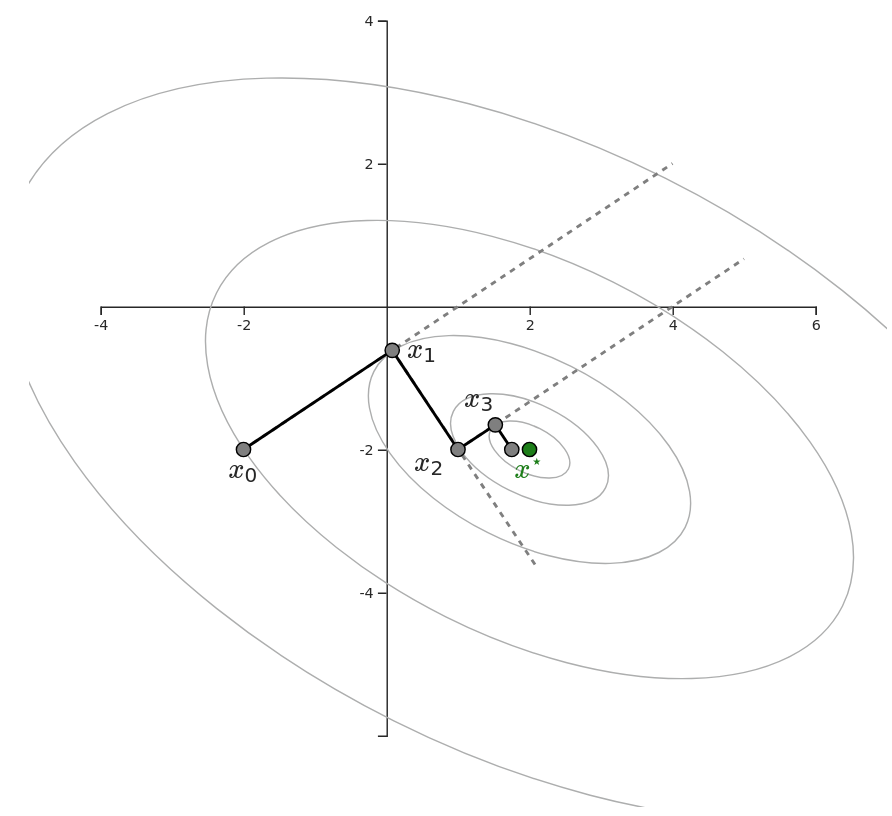
\includegraphics[width=0.7\textwidth]{./atelier/img/gradient_descent.png}
\caption{Approximation des Minimierers einer Funktion $F$ in zwei Variablen mit Hilfe des adaptiven Gradientenverfahrens \eqref{eq:gradient_descent_adaptive}.}
\label{fig:gradient_descent_adaptive}
\end{figure}
In Abbildung \ref{fig:gradient_descent_adaptive} ist ein typischer Verlauf des adaptiven Gradientenverfahrens in Algorithmus \ref{alg:gradient_descent_adaptive} bei der Minimierung einer Funktion $F \colon \mathbb{R}^2 \rightarrow \mathbb{R}$ zu sehen. 
Man erkennt, dass die Schrittweiten immer kleiner werden, je näher man sich dem lokalen Minimum $x_*$ nähert.
Außerdem sieht man, dass die Richtung des steilsten Gradientenabstiegs immer orthogonal zu den Niveaulinien der zu minimierenden Funktion steht.

\begin{remark}{}{}
Das in diesem Abschnitt beschriebene Gradientenabstiegsverfahren mit adaptiver Schrittweite $\tau_k > 0$ ist ein gängiger Algorithmus zur Minimierung einer Funktion $F$, wenn deren Ableitung $\nabla F$ bekannt und numerisch günstig zu berechnen ist. 
Dennoch gibt es Situationen in denen es ratsam ist alternative Optimierungsalgorithmen zu verwenden. 
Zum Beispiel ist ein häufiges Problem des Gradientenverfahrens die starke Verlangsamung in der Nähe eines Sattelpunktes, was zu sehr langen Laufzeiten des Algorithmus führt. 
Außerdem passiert die Minimierung einer Funktion $F$ mit Hilfe des Gradientenabstiegsverfahrens in der Regel entlang eines Zickzack-Pfades (siehe Abbildung \ref{fig:gradient_descent_adaptive}), welcher in den meisten Fällen offensichtlich suboptimal ist. 
Aus diesen Gründen wollen wir uns in den nächsten Abschnitten mit alternativen Minimierungsmethoden beschäftigen.
\end{remark}

\subsection{Koordinatenabstiegsverfahren}
\label{ss:coordinate_descent}
Eine weitere Variante des in Kapitel \ref{ss:gradient_descent} behandelten Gradientenabstiegsverfahrens ist das \textit{Koordinatenabstiegsverfahren} (im Englischen: \textit{coordinate descent} (CD)). 

Die grundlegende Idee des Koordinatenabstiegsverfahrens ist es in jedem Schritt des Iterationsschemas eine \textit{Koordinatenrichtung} auszuwählen und einen Abstieg in diese Richtung durchzuführen. 
Damit lässt sich ein möglicherweise kompliziertes multivariates Optimierungsproblem durch eine Reihe von einfachen univariaten Optimierungsproblemen behandeln.
Die Auswahl der Koordinatenrichtung kann entweder mit Hilfe einer Auswahlregel, z.B. mit einem Rundlaufverfahren, oder aber zufällig geschehen.

Wir wollen im Folgenden den Fall einer zufälligen Wahl der Koordinatenrichtung diskutieren.
Für einen zufälligen Index $j \in \lbrace 1,\ldots,n\rbrace$ und den entsprechenden zufälligen Einheitsvektor $\vec{e}_j \in \mathbb{R}^n$ lässt sich das Koordinatenabstiegsverfahren schreiben als:
\begin{equation}
\label{eq:coordinate_descent_stochastic}
x_{k+1} \ = \ x_k - \alpha_k \langle \nabla F(x_k), \vec{e_j} \rangle \vec{e_j} \ = \ x_k - \frac{\partial F}{\partial x^i}(x_k) \vec{e_j}.
\end{equation}
Das bedeutet, dass man in jeder Iteration nur eine Koordinate des aktuellen Parametervektors $x_k \in \Omega$ verändern muss.
Die Schrittweite $\alpha_k > 0$ in \eqref{eq:coordinate_descent_stochastic} kann hierbei ähnlich wie in Kapitel \ref{ss:gradient_descent} fest oder adaptiv gewählt werden.
Das Koordinatenabstiegsverfahren in \eqref{eq:coordinate_descent_stochastic} mit adaptiver Schrittweite lässt sich mit folgendem Algorithmus umsetzen.

~\\
\begin{algorithm}{Koordinatenabstiegsverfahren}{}
\label{alg:coordinate_descent_stochastic}
\begin{algorithmic}
\STATE \textbf{function} $[x^*, F(x^*)]= $\texttt{coordinateDescentStochastic}$(F,\nabla F, x_0, \alpha_0, \sigma, \epsilon$) \{
\STATE ~
\STATE \# Initialisierung
\STATE $\alpha_k = \alpha_0$
\STATE $x_k = x_0$
\STATE $F(x_{k+1}) = +$\texttt{Inf}
\STATE ~
\STATE \# Iteriere bis gewünschte Genauigkeit erreicht ist
\WHILE{$F(x_{k+1}) - F(x_k) > \epsilon$}
\STATE \# Wähle zufällige Koordinatenrichtung
\STATE $i = \texttt{randomDraw}([1:n])$
\STATE \# Berechne Richtungsableitung
\STATE $\vec{p}_k = \frac{\partial}{\partial x^i}F(x_k)$
\WHILE{$ F(x_k - \alpha_k \vec{p}_k / ||\vec{p}_k|| ) > F(x_k)$}
%\STATE ~
\STATE \# Verringere Schrittweite um Faktor $\sigma$
\STATE $\alpha_k = \sigma\alpha_k$
%\STATE ~
\ENDWHILE
\STATE \# Update in Richtung des größten Gradientenabstiegs
\STATE $x_{k+1} = x_k - \alpha_k \vec{p}_k / ||\vec{p}_k|| $
%\STATE ~
\ENDWHILE
\STATE ~
\STATE \# Ausgabe des letzten Punktes
\STATE $x^* = x_k$
\STATE $F(x^*) = F(x_k)$
\STATE \}
\end{algorithmic}
\end{algorithm}

%\textbf{ToDo: Abbildung erstellen}

Das Koordinatenabstiegsverfahren benötigt in der Regel deutlich mehr Iterationen als das normale Gradientenabstiegsverfahren und beschreibt häufig noch mehr einen Zickzack-Pfad bei der Minimierung.%, wie man in Abbildung \ref{fig:coordinate_descent_stochastic} sehen kann.
Dennoch bietet das Verfahren Vorteile gegenüber dem Gradientenabstiegsverfahren gerade in Optimierungsproblemen mit vielen Variablen, da jedes eindimensionale Optimierungsproblem wesentlich leichter zu lösen ist als die Berechnung des gesamten Gradienten in jedem Schritt. 

\begin{remark}{}{}
Um den Zufallseffekten und den damit verbundenen Zickzack Pfad bei der Minimierung der Funktion $F$ durch das Koordinatenabstiegsverfahren entgegen zu wirken, kann man einen Kompromiss zwischen der Verwendung einer einzelnen Koordinatenrichtung und dem gesamten Gradienten eingehen. 
Hierbei spricht man von den sogenannten \textit{Blockkoordinatenabtiegsverfahren} (im Englischen \textit{block coordinate descent} (BCD)).
Hierbei wählt man zuerst die Größe $s \in \lbrace 1,\ldots,n\rbrace$ der Koordinatenblöcke, d.h., die Größe der Teilmenge der verwendeten Richtungsableitungen des Gradienten $\nabla F$. Anschließend wird in jedem Schritt ein Block an Koordinatenrichtungen deterministisch oder zufällig ausgewählt und in dessen Richtung minimiert.
Für eine zufällige Wahl der Koordinatenblöcke ergibt sich somit:
\begin{equation}
\label{eq:block_coordinate_descent}
x_{k+1} \ = \ x_k - \alpha_k \langle \nabla F(x_k), \sum_{i=1}^s\vec{e}_{\sigma(i)} \rangle \sum_{i=1}^s\vec{e}_{\sigma(i)}.
\end{equation}
Hierbei ist $\sigma \colon \lbrace1,\ldots,n\rbrace \rightarrow \ \lbrace1,\ldots,n\rbrace$ eine zufällige Permutation der Indizes $1,\ldots,n$.
Es ist klar, dass das Koordinatenabstiegsverfahren in \eqref{eq:coordinate_descent_stochastic} und das normale Gradientenabstiegsverfahren in \eqref{eq:gradient_descent_adaptive} Spezialfälle des Blockkoordinatenabstiegsverfahrens in \eqref{eq:block_coordinate_descent} für Blockgrößen $s = 1$ und $s=n$ sind.
\end{remark}

\subsection{Stochastisches Gradientenabstiegsverfahren}
\label{ss:stochastic_gradient_descent}
Eine aktuell weit verbreitete Variante des Gradientenabstiegsverfahrens in \eqref{eq:gradient_descent_adaptive} ist das \textit{stochastische Gradientenabstiegsverfahren} (im Englischen: \textit{stochastic gradient descent} (SGD)). 
Wie der Name schon verrät handelt es sich hierbei nicht um einen deterministischen Algorithmus.
Das bedeutet, dass man bei mehrmaliger Anwendung des Verfahrens bei gleichbleibenden Startbedingungen in der Regel unterschiedliche Ergebnisse in unterschiedlichen Laufzeiten erhält.
Was auf den ersten Blick wie ein Nachteil wirkt, kann in manchen Fällen jedoch praktische Eigenschaften mit sich bringen.
So kann die Zufallsnatur des stochastischen Gradientenverfahrens dazu führen, dass Sattelpunkte und schlechte, lokale Minima der Funktion durch die Folge der Punkte vermieden werden.
Das Verfahren findet aktuell vor allem beim Training von neuronalen Netzen bei der sogenannten \textit{Backpropagation} in verschiedenen Variationen Anwendung, da man hierdurch dem bekannten Problem des \textit{Übertrainierens} des neuronalen Netzes entgegen wirken kann.

Beim stochastischen Gradientenverfahren geht man davon aus, dass sich die zu minimierende Zielfunktion $F \colon \Omega \rightarrow \mathbb{R}$ als eine Summe der folgenden Gestalt schreiben lässt:
\begin{equation}
\label{eq:objective_function_sum}
F(x) \ = \ \sum_{i=1}^m F_i(x), \quad \text{ für alle } x \in \Omega.
\end{equation} 
Solche Zielfunktionen treten natürlicherweise in vielen Problemstellungen auf, zum Beispiel bei Maximimum-Likelihood Ansätzen oder der Methode der kleinsten Quadrate.
Im Bereich des maschinellen Lernens lässt sich der Trainingsfehler über alle Trainingsdaten in der Regel als eine solche Summe  schreiben.
In diesem Fall lässt sich das normale Gradientenabstiegsverfahren in \eqref{eq:gradient_descent_adaptive} umschreiben zu:
\begin{equation}
\label{eq:gradient_descent_sum}
x_{k+1} \ = \ x_k - \alpha_k \frac{\nabla F(x_k)}{||\nabla F(x_k)||} \ = \ x_k - \alpha_k \frac{\sum_{i=1}^m\nabla F_i(x_k)}{||\sum_{i=1}^m\nabla F_i(x_k)||}, \quad \alpha_k > 0 .
\end{equation}

Die Idee des stochastischen Gradientenverfahrens ist es nun einen zufälligen Summanden aus \eqref{eq:objective_function_sum} zu wählen und nur den Gradienten bezüglich dieses Summanden zu betrachten.
Durch diese starke Vereinfachung von \eqref{eq:gradient_descent_sum} führt man mit einem zufällig ausgewählten Index $j \in \lbrace 1,\ldots,m\rbrace$ nun einen Gradientenabstieg der Form
\begin{equation}
\label{eq:stochastic_gradient_descent}
x_{k+1} \ = \ x_k - \alpha_k \frac{\nabla F_j(x_k)}{||\nabla F_j(x_k)||}, \quad \alpha_k > 0
\end{equation}
durch.
\begin{remark}{}{}
Ähnlich wie im Fall des Koordinatenabstiegsverfahrens in Kapitel \ref{ss:coordinate_descent}, gibt es auch beim stochastischen Gradientenverfahren die Möglichkeit einen Kompromiss zwischen dem normalen Gradientenabstieg in \eqref{eq:gradient_descent_control} und dem auf einen Summanden beschränkten Gradientenabstieg \eqref{eq:stochastic_gradient_descent} einzugehen. 
Indem man eine zufällige Untermenge von fester Größe $s \in \lbrace 1,\ldots,m\rbrace$ von Summanden von $F$ auswählt, lässt sich das sogenannte \textit{stochastische Minibatch-Gradientenabstiegsverfahren} formulieren:
\begin{equation*}
x_{k+1} = x_k - \alpha_k \frac{\sum_{i=1}^s\nabla F_{\sigma(i)}(x_k)}{||\sum_{i=1}^s\nabla F_{\sigma(i)}(x_k)||}, \quad \alpha_k > 0 .
\end{equation*}
Hierbei ist $\sigma \colon \lbrace 1,\ldots,m\rbrace \rightarrow \lbrace 1,\ldots,m\rbrace$ eine zufällige Permutation der Indizes $1,\ldots,m$.
\end{remark}

\subsection{Newton Verfahren}
\label{ss:newton}
In diesem Abschnitt wollen wir uns das bereits bekannte Newton-Verfahren in Erinnerung rufen und dieses geeignet zur Optimierung von nichtlinearen Funktionen verallgemeinern. 
In Kapitel $5.1$ der Vorlesung \glqq Einführung in die Numerik\grqq haben wir das Newton Verfahren zur Approximation von Nullstellen nichtlinearer Gleichungssysteme hergeleitet. 
Aus der Taylorentwicklung einer nichtlinearen Nullstellengleichung $F(x^*) = 0$ von der Form
\begin{equation*}
0 \ = \ F(x^*) \ = \ F(x) + (x^* - x) F'(x) + \mathcal{O}(F'').
\end{equation*}
haben wir die folgende Fixpunktfunktion als Approximation erster Ordnung angegeben: 
\begin{equation}
\label{eq:newton_fixpunkt}
G(x) \ = \ x - (F'(x))^{-1} F(x), \quad \text{ für } F'(x) \neq 0.
\end{equation}
Hierbei haben wir die Fixpunktgleichung als erfüllt gesehen, wenn wir ein $x^* \in \Omega$ gefunden haben, so dass die linke und rechte Seite von \eqref{eq:newton_fixpunkt} übereinstimmen. Unter dieser Beobachtung haben wir das \textit{Newton-Verfahren} als iteratives Schema zur Bestimmung eines solchen Fixpunktes $x^* \in \Omega$ hergeleitet:
\begin{equation}
x_{k+1} \ = \ x_k - \frac{F(x_k)}{F'(x_k)}.
\end{equation}
Hierfür benötigten wir einen geeigneten Startwert $x_0 \in \Omega$ in einer lokalen Umgebung $U \subset \Omega$ des Fixpunktes $x^* \in U$. Der folgende Satz Bedingungen für die lokale Konvergenz des Newton-Verfahrens. 
\begin{theorem}{}{}
Sei $F: \R^n \rightarrow \R^n$ in einer Umgebung von $\overline{x}$ stetig differenzierbar,  $F'$ lokal Lipschitz stetig , $F(\overline{x}) = 0$ und  $F'(\overline{x})$  regul\"ar. Dann existiert eine Umgebung $B_R(\overline{x})$, sodass das Newton-Verfahren f\"ur jeden Startwert $x_0 \in B_R(\overline{x})$ konvergiert, d.h. $x_k \rightarrow \overline{x}$.
\end{theorem}
\begin{proof}
Siehe \cite[Satz 5.7]{numerik1}.
\end{proof}

Anstatt nun eine Nullstelle der Funktion $F$ zu suchen, wollen wir das Newton-Verfahren nutzen, um eine Nullstelle des Gradienten $\nabla F$, d.h. einen stationären Punkt zu approximieren und damit die notwendigen Optimalitätsbedingungen zu erfüllen.
Im Folgenden sei $\Omega \subset \mathbb{R}^n$ ein offenes, zusammenhängendes Gebiet und $F \colon \Omega \rightarrow \mathbb{R}$ eine differenzierbare, reellwertige Funktion.
Wir betrachten wieder die Taylorapproximation der Funktion $F$ in eine Abstiegsrichtung $x_k + \vec{p} \in \Omega$ des allgemeinen Iterationsschemas \eqref{eq:abstiegsverfahren} aber berücksichtigen diesmal auch Terme von zweiter Ordnung:
\begin{equation}
\label{eq:modellfunktion}
F(x_k + \vec{p}) \ \approx \ F(x_k) + \langle \vec{p}, \nabla F(x_k) \rangle + \frac{1}{2} \langle \vec{p}, \nabla^2F(x_k)\vec{p} \rangle \ \eqqcolon \ m_k(\vec{p}).
\end{equation}
Wenn wir für den Moment davon ausgehen, dass die Hessematrix $\nabla^2 F(x_k)$ positiv definit ist, so können wir ein eindeutiges Minimum der Funktion $m_k(\vec{p})$ wie folgt bestimmen:
\begin{equation}
\label{eq:newton_richtung}
\vec{p} \ = \ -(\nabla^2 F(x_k))^{-1} \nabla F(x_k).
\end{equation}
Die Richtung $\vec{p} \in \mathbb{R}^n / \lbrace 0 \rbrace$ in \eqref{eq:newton_richtung} wird auch \emph{Newton-Richtung} genannt.
Mit ihr lässt sich ein iteratives Abstiegsverfahren für einen initialen Punkt $x_0 \in \Omega$, welcher geeignet in der Nähe des stationären Punktes $x^* \in \Omega$ gewählt wird, wie folgt konstruieren:
\begin{equation}
\label{eq:newton_abstieg}
x_{k+1} \ = \ x_k + \vec{p} \ = \ x_k - (\nabla^2 F(x_k))^{-1} \nabla F(x_k).
\end{equation}
Damit das Newton-Abstiegsverfahren in \eqref{eq:newton_abstieg} überhaupt sinnvoll ist, müssen wir fordern, dass die Hessematrix in jedem Punkt $x_k \in \Omega$ der Iterationsfolge invertierbar ist.
Um sicher zu gehen, dass es sich tatsächlich um eine Abstiegsrichtung handelt müssen wir fordern, dass die Hessematrix $\nabla^2 F(x_k)$ nicht nur invertierbar für alle $x_k \in \Omega$ der Iterationsfolge ist, sondern auch positiv definit in jedem Punkt $x_k$ ist. Denn dann ergibt eine Taylorapproximation zweiter Ordnung die folgende Abschätzung:
\begin{equation*}
\begin{split}
F(x_{k+1}) \ &= \ F(x_k + \vec{p}) \ \approx \ F(x_k) + \langle p, \nabla F(x_k) \rangle + \frac{1}{2} \langle \vec{p}, \nabla^2F(x_k) \vec{p} \rangle \\
\ &= \ F(x_k) - \langle (\nabla^2 F(x_k))^{-1} \nabla F(x_k), \nabla F(x_k) \rangle + \frac{1}{2} \langle \vec{p}, \nabla^2F(x_k) \vec{p} \rangle\\
\ &= \ F(x_k) - \langle (\nabla^2 F(x_k))^{-1} \nabla^2 F(x_k) \vec{p}, \nabla^2 F(x_k) \vec{p} \rangle + \frac{1}{2} \langle \vec{p}, \nabla^2F(x_k) \vec{p} \rangle \\
\ &= \ F(x_k) - \frac{1}{2} \underbrace{\langle \vec{p}, \nabla^2 F(x_k) \vec{p}}_{>~0} \rangle.
\end{split}
\end{equation*}
Wir sehen also, dass wir einen echten Abstieg der Funktionswerte erhalten, wenn die Hessematrix $\nabla^2 F(x_k)$ positiv definit ist für alle $x_k \in \Omega$ der Iterationsfolge. 
Sollte die Hessematrix nicht positiv definit in einem Punkt $x_k$ der Iterationsfolge sein, so muss zumindest eine Abnahme der Funktionswerte vorliegen, d.h., es muss für die Newton-Abstiegsrichtung gelten:
\begin{equation*}
\langle (\nabla^2F(x_k))^{-1} \nabla F(x_k), \nabla F(x_k) \rangle \ > \ 0.
\end{equation*}
Sollte dies nicht der Fall sein, so existieren Methoden um dennoch einen Abstieg zu erzwingen, siehe zum Beispiel \cite[Kapitel 6]{nocedal_1999}. Auf diese werden wir jedoch im weiteren Verlauf der Vorlesung nicht näher eingehen.
\begin{remark}{}{}
Das Newton-Abstiegsverfahren in \eqref{eq:newton_abstieg} ist ein Abstiegsverfahren der Art \eqref{eq:abstiegsverfahren} dessen Schrittweite $\alpha_k$ durch die lokale Krümmung und die Ableitung der Funktion $F$ bestimmt ist. In diesem Fall können wir $\alpha_k \equiv 1$ für alle $k \in \mathbb{N}$ setzen.
Das Newton-Abstiegsverfahren konvergiert in der Regel \emph{quadratisch} gegen einen stationären Punkt $x^* \in \Omega$ mit $\nabla F(x^*)=0$, d.h. man erreicht sehr schnell eine hohe Genauigkeit bei der Approximation von $x^*$.
\end{remark}

\subsection{Quasi-Newton Verfahren}
\label{ss:quasi-newton}
Im Kapitel \ref{ss:newton} haben wir das Newton Verfahren zur iterativen Approximation eines stationären Punktes $x^* \in \Omega$ einer Funktion $F$ mit $\nabla F(x^*) = 0$ hergeleitet. 
Hierbei haben wir im Gegensatz zu den vorherigen numerischen Verfahren auch Ableitungen höherer Ordnung hinzugezogen. 
Dies führt in der Regel zu einem verbesserten Konvergenzverhalten im Vergleich zu den Verfahren, die nur die lokale Ableitung $\nabla F$ der Funktion $F$ verwenden.
Dennoch ist das Newton Verfahren aus numerischer Sicht noch nicht ideal, da einige Probleme mit sich bringt.
Zuerst mussten wir fordern, dass die Hessematrix $\nabla^2 F(x_k)$ in jedem Punkt des Iterationsverfahrens positiv definit ist, da ansonsten kein Abstieg der Funktionswerte garantiert werden kann.
Zweitens muss für die Berechnung der Newton-Richtung in \eqref{eq:newton_richtung} zuerst die Hessematrix bestimmt und anschließend invertiert werden.
Dies ist aus Effizienzgründen ungewünscht, da die Inversion einer $n \times n$-Matrix in $\mathcal{O}(n^3)$ Rechenoperationen liegt.
Da die Bestimmung und die Inversion der Hessematrix in jedem Iterationsschritt passieren müssen, ist das Newton Verfahren nicht empfehlenswert für die numerische Optimierung.

Eine naheliegende Idee ist es nun die echte Hessematrix in jedem Iterationsschritt durch eine geeignete Matrix zu approximieren, so dass der numerische Aufwand geringer wird, d.h., wir suchen nach einer Matrix
\begin{equation}
\label{eq:matrix_bk}
B_k \approx \nabla^2 F(x_k).
\end{equation}
Damit können wir die Modellfunktion $m_k(\vec{p})$ in \eqref{eq:modellfunktion} schreiben als:
\begin{equation*}
m_k(\vec{p}) \ = \ F(x_k) + \langle \nabla F(x_k), \vec{p} + \frac{1}{2} \langle \vec{p}, B_k \vec{p} \rangle,
\end{equation*}
das heißt, wir approximieren die Zielfunktion $F$ im $k$-ten Iterationsschritt entlang der Richtung $\vec{p} \in \mathbb{R}^n$ lokal durch eine quadratische Funktion.
Für sehr kleine Schrittweiten können wir davon ausgehen, dass der Fehler dieser Approximation gering ist, da wir davon ausgehen, dass $F$ stetig differenzierbar in einer lokalen Umgebung $U \subset \Omega$ des stationären Punktes $x^* \in \Omega$ ist und für $\vec{p} = 0$ die Approximation exakt ist, da
\begin{equation*}
m_k(0) \ = \ F(x_k).
\end{equation*}
Wenn wir fordern, dass $B_k$ in \eqref{eq:matrix_bk} eine positiv definite Matrix ist, so lässt sich ein Abstiegsschritt des Iterationsverfahrens \eqref{eq:abstiegsverfahren} analog zur Herleitung des Newton Abstiegsverfahrens in Kapitel \ref{ss:newton} angeben als:
\begin{equation}
\label{eq:quasi-newton-abstieg}
x_{k+1} \ = \ x_k + \alpha_k \vec{p}_k, \qquad \vec{p}_k \ = \ -B_k^{-1} \nabla F(x_k).
\end{equation}
Die sogenannten \emph{Quasi-Newton Verfahren} verfolgen diesen Ansatz. 
Durch die Approximation der echten Hessematrix verlieren Quasi-Newton Verfahren an Genauigkeit, wodurch ihre Konvergenzgeschwindigkeit superlinear anstatt quadratisch ist. 
Dafür gewinnen sie zusätzliche Geschwindigkeit durch die Vermeidung der Bestimmung und Inversion von $\nabla^2 F(x_k)$.
Der Vorteil der Quasi-Newton Methoden ist es, dass man nur den Gradienten $\nabla F$ für einen Schritt des numerischen Optimierungsverfahrens benötigt und keine expliziten Informationen über die zweiten Ableitungen.
Dadurch werden sie in bestimmten Problemen sogar effizienter bei der Approximation eines stationären Punktes als das Newton Abstiegsverfahren in Kapitel \ref{ss:newton}.

Die entscheidende Frage bei der Konstruktion eines Quasi-Newton Abstiegsverfahrens der Form \eqref{eq:quasi-newton-abstieg} ist es, wie die positiv definite Matrix $B_k$ in jedem Schritt möglichst effizient bestimmt werden kann. 
Anstatt die Näherung $B_k$ der Hessematrix $\nabla^2 F(x_k$ in jedem Schritt von Grund auf neu zu berechnen, wäre es wünschenswert ein initiales $B_0$ in jedem Schritt des Iterationsverfahrens zu aktualisieren.
Hierbei ist es möglich die durch den Iterationsschritt erhaltenen Informationen über den Gradienten $\nabla F$ zu Hilfe zu nehmen.
Wir nehmen an, wir haben bereits einen Abstiegsschritt durchgeführt und so einen neuen Punkt $x_{k+1} = x_k + \alpha_k\vec{p}$ erhalten.
Unsere quadratische Approximation in diesem neuen Punkt für eine neue Richtung $\vec{p} \in \mathbb{R}^n$ sieht dementsprechend wie folgt aus:
\begin{equation*}
m_{k+1}(\vec{p}) \ = \ F(x_{k+1}) + \langle \nabla F(x_{k+1}), \vec{p} \rangle + \frac{1}{2}\langle \vec{p}, B_{k+1}\vec{p} \rangle.
\end{equation*}
Eine Forderung, die man nun die Modellfunktion $m_{k+1}$ stellen kann ist, dass ihre Ableitung mit der Ableitung der Zielfunktion $F$ in den letzten beiden Punkten $x_k$ und $x_{k+1}$ übereinstimmt.
Da
\begin{equation*}
\nabla m_{k+1}(0) \ = \ \nabla F(x_{k+1})
\end{equation*}
gilt, ist eine der beiden Forderungen automatisch erfüllt.
Für die zweite Forderung können wir nutzen, dass $x_k = x_{k+1} - \alpha_k \vec{p}_k$ gilt und wir somit erhalten:
\begin{equation}
\label{eq:quasi-newton_forderung}
\nabla m_{k+1}(-\alpha_k\vec{p}_k) \ = \ \nabla F(x_{k+1}) - \alpha_k B_{k+1}\vec{p}_k \ \overset{!}{=} \ \nabla F(x_k).
\end{equation}
Durch Umstellen von \eqref{eq:quasi-newton_forderung} erhalten wir die Bedingung
\begin{equation*}
B_{k+1}\alpha_k \vec{p}_k \ = \ B_{k+1}(x_{k+1} - x_k) \ \overset{!}{=} \ \nabla F(x_{k+1}) - \nabla F(x_k).
\end{equation*}
Eine vernünftige Wahl der Matrix $B_{k+1}$ in \eqref{eq:matrix_bk} sollte diese Eigenschaft, auch bekannt als \textbf{Sekantengleichung}, versuchen zu imitieren.
Im eindimensionalen Fall mit $F \colon \Omega \subset \mathbb{R} \rightarrow \mathbb{R}$ bedeutet die Sekantengleichung nichts anderes, als dass der Faktor $B_{k+1}$ eine Approximation des zweiten Ableitung von $F$ im Sinne eines Differenzenquotienten ist, d.h., im Fall $n=1$ soll gelten:
\begin{equation*}
B_{k+1} \ \overset{!}{=} \ \frac{F'(x_{k+1})-F'(x_k)}{x_{k+1} - x_k}.
\end{equation*}

Für unser allgemeines Quasi-Newton Verfahren in \eqref{eq:quasi-newton-abstieg} suchen wir also einen Weg die bereits bekannte Approximation der Hessematrix $B_k \approx \nabla^2F(x_k)$ zu einer Matrix $B_{k+1}$ aktualisieren, so dass der folgende Zusammenhang für den nächsten Punkt $x_{k+1} \in \Omega$ erfüllt wird:
\begin{equation}
\label{eq:sekantengleichung}
B_{k+1} s_k \ = \ y_k,
\end{equation}
wobei
\begin{equation*}
s_k \ = \ x_{k+1} - x_k, \qquad y_k = \nabla F(x_{k+1}) - \nabla F(x_k).
\end{equation*}
Es wird klar, dass diese Forderung alleine nicht genügt für die Konstruktion eines Abstiegsverfahrens.
Um die positive Definitheit der Matrix $B_{k+1}$ in Schrittrichtung $\alpha\vec{p}_k$ zu gewährleisten müssen wir fordern, dass die Vektoren $y_k$ und $s_k$ die sogenannte \textbf{Krümmungsbedingung} erfüllen:
\begin{equation}
\label{eq:kruemmungsbedingung}
\langle s_k, y_k \rangle \ > \ 0.
\end{equation}
Dies ist eine hinreichende Bedingung für die positive Definitheit von $B_{k+1}$ bezüglich der Richtung $\alpha_k \vec{p}_k$, da wir einfach die Sekantengleichung \eqref{eq:sekantengleichung} von links mit dem Vektor $s_k^T$ multiplizieren können und so erhalten wir mit der Forderung \eqref{eq:kruemmungsbedingung} schon:
\begin{equation*}
\langle s_k, B_{k+1}s_k \rangle \ = \ \langle s_k, y_k \rangle \ > \ 0.
\end{equation*}
\begin{remark}{}{}
Falls die Funktion $F$ strikt konvex ist, so ist die Krümmungsbedingung \eqref{eq:kruemmungsbedingung} für alle Punktepaare $x_k, x_{k+1} \in \Omega$ erfüllt und die Matrix $B_{k+1}$ wird damit positiv definit. Für nichtkonvexe Funktionen hingegen muss man die Krümmungsbedingung explizit forcieren, um ein Abstiegsverfahren zu erhalten.
\end{remark}

Falls die Krümmungsbedingung \eqref{eq:kruemmungsbedingung} erfüllt ist, so existiert mindestens eine Lösung $B_{k+1}$ der Sekantengleichung \eqref{eq:sekantengleichung}.
Man sieht ein, dass es in der Tat sogar unendlich viele Lösungen $B_{k+1}$ gibt, da eine symmetrische $n \times n$ Matrix $n(n+1)/2$ Freiheitsgrade besitzt und die Sekantengleichung \eqref{eq:sekantengleichung} nur $n$ Bedingungen an $B_{k+1}$ stellt.
Zusätzlich erhält man $n$ Bedingungen an $B_{k+1}$ durch die Forderung von positiver Definitheit, da alle $n$ Hauptminoren von $B_{k+1}$ positiv sein müssen.
Dies reicht jedoch nicht für die eindeutige Bestimmung der Matrix $B_{k+1}$.
Hierfür müssen wir zusätzlich fordern, dass die Matrix $B_{k+1}$ diejenige Matrix unter allen möglichen Lösungen ist, die der vorherigen Matrix $B_k$ am nächsten bezüglich eines geeigneten Maßes ist.
Das heißt wir suchen eine Lösung des folgenden Optimierungsproblems:
\begin{equation}
\label{eq:quasi-newton_optimization-problem}
\begin{split}
\min_{B} || B - B_k ||, \quad \text{ unter den Nebenbedingungen: } \\
B \ = \ B^T, \qquad B s_k \ = \ y_k, \qquad \langle \vec{p}, B\vec{p} \rangle > 0, \forall \vec{p} \in \mathbb{R}^n / \lbrace 0 \rbrace,
\end{split}
\end{equation}
wobei $s_k$ und $y_k$ definiert sind wie in der Sekantengleichung \eqref{eq:sekantengleichung}.
Man beachte, dass man eine unterschiedliche Lösung $B_{k+1}$ des Optimierungsproblems \eqref{eq:quasi-newton_optimization-problem} in Abhängigkeit der gewählten Matrixnorm erhält und somit auch ein unterschiedliches Quasi-Newton Verfahren herleiten kann.

\subsubsection{Das Davidon-Fletcher-Powell Verfahren}
Im ursprünglich im Jahr $1959$ von Davidon vorgeschlagenen Verfahren \cite{davidon_1959}, das im Übrigen bei der Erstbegutachtung abgelehnt wurde, wählt man für die Norm im Optimierungsproblem \eqref{eq:quasi-newton_optimization-problem} eine gewichtete Frobeniusnorm der Form
\begin{equation*}
||A||_W \ \coloneqq \ || W^\frac{1}{2}A W^\frac{1}{2} ||_F.
\end{equation*}
Die Gewichtungsmatrix $W$ dient dazu, dass das implizierte Quasi-Newton Verfahren zur Approximation eines stationären Punktes $x^* \in \Omega$ skalierungs-invariant wird. 
Hierzu wählt man eine beliebige Matrix für die die Relation $W y_k = s_k$ gilt, d.h., eine Matrix $W$, die sich wie die Inverse der Matrix $B$ in \eqref{eq:quasi-newton_optimization-problem} verhält.
Ein konkretes Beispiel solch eine Gewichtungsmatrix wäre $W \coloneqq G_k^{-1}$, wobei $G_k$ die durchschnittliche Hessematrix von $F$ entlang des letzten Abstiegsschritts von $x_k \rightarrow x_{k+1}$ ist mit
\begin{equation*}
G_k \ \coloneqq \ \int_0^1 \nabla^2 F(x_k + t \alpha_k \vec{p}_k)~\mathrm{d}t.
\end{equation*}
Mit der konkreten Wahl dieser Gewichtungsmatrix $W = G_k^{-1}$ wird die gewichtete Frobeniusnorm  dimensionslos und man erhält eine eindeutige Lösung des Optimierungsproblems \eqref{eq:quasi-newton_optimization-problem} wie folgt:
\begin{equation}
\label{eq:DFP}
B_{k+1} \ = \ (I-\gamma_k y_ks_k^T) B_k (I - \gamma_k s_k y_k^T) + \gamma_k y_k y_k^T, \quad \text{ mit } \gamma_k \ \coloneqq \ \frac{1}{\langle y_k, s_k \rangle}.
\end{equation}
Die Gleichung \eqref{eq:DFP} wird auch \textbf{DFP-Schritt} genannt, da sie zuerst von Davidon vorgeschlagen und später von Fletcher und Powell untersucht und verbreitet wurde.

Obwohl wir die explizite Berechnung der Hessematrix $\nabla^2 F(x_k)$ vermieden haben und die Aktualisierung der Matrix $B_k$ zu $B_{k+1}$ lediglich auf den Gradienteninformationen von $F$ basiert ist der numerische Aufwand bei direkter Verwendung von $B_{k+1}$ in \eqref{eq:DFP} noch zu hoch.
Das liegt daran, dass wir für einen Schritt des Quasi-Newton Verfahrens in \eqref{eq:quasi-newton-abstieg} die Inverse der Matrix $B_k$ benötigen und die Inversion einen numerischen Aufwand von $\mathcal{O}(n^3)$ besitzt.
Glücklicherweise gibt es einen Trick, wie wir die Inverse von $B_k$ in jedem Schritt des Iterationsverfahrens numerisch günstig erhalten können.
Sei $H_k \coloneqq B_k^{-1}$, dann können wir die sogenannte Sherman-Morrison-Woodbury Formel auf Gleichung \eqref{eq:DFP} anwenden um die neue Inverse $H_{k+1}$ durch eine Aktualisierung der Matrix $H_k$ zu berechnen:
\begin{equation}
\label{eq:smw-formel}
H_{k+1} \ = \ H_k - \frac{H_k y_k y_k^T H_k}{\langle y_k, H_k y_k\rangle} + \frac{s_k s_k^T}{\langle y_k, s_k \rangle} . 
\end{equation}
Wie man einssieht liegt der numerische Rechenaufwand für das Update von $H_{k+1}$ in \eqref{eq:smw-formel} in $\mathcal{O}(n^2)$.
Es fällt außerdem auf, dass $H_k$ nur durch die Addition zweier Matrizen mit Rang $1$ verändert wird, also insgesamt eine Änderung von höchstes Rang $2$ erfährt.
Das passt gut zu der Forderung, dass wir erwarten, dass sich die Approximation der Hessematrix $\nabla^2 F$ in einer lokalen Umgebung nur wenig ändert.

\subsubsection{Das Broyden--Fletcher--Goldfarb--Shanno Verfahren}
Das Davidon--Fletcher--Powell Verfahren wurde trotz seiner Effektivität bald schon durch ein Verfahren abgeläst, dass noch besser war und bis heute zu den effizientesten Quasi-Newton Verfahren gehört: das Broyden--Fletcher--Goldfard--Shanno (BFGS) Verfahren.
Die Idee des BFGS Verfahrens leitet sich unmittelbar aus der Idee des DFP Verfahren ab.
Anstatt das Optimierungsproblem \eqref{eq:quasi-newton_optimization-problem} mit bestimmten Bedingungen an die Approximation $B_{k+1}$ der Hessematrix $\nabla^2 F(x_k)$ zu stellen, versucht man direkt die Inverse der Hessematrix $(\nabla^2 F(x_k))^{-1}$ geeignet zu approximieren.
Hierfür nehmen wir an, dass wir eine Matrix $H_{k+1}$ als geringfügige Aktualisierung einer bereits vorher bestimmten Matrix $H_k$ suchen, die gleichzeitig symmetrisch und positiv definit ist und zusätzlich die Sekantenbedingung in umgeschriebener Form erfüllt:
\begin{equation*}
H_{k+1}y_k \ = \ s_k.
\end{equation*}
Hierzu formuliert man ein analoges Optimierungsproblem zu \eqref{eq:quasi-newton_optimization-problem} von der Form:
\begin{equation}
\label{eq:bfgs_optimierungsproblem}
\begin{split}
\min_{H} || H - H_k ||, \quad \text{ unter den Nebenbedingungen: } \\
H \ = \ H^T, \qquad H y_k \ = \ s_k, \qquad \langle \vec{p}, H\vec{p} \rangle > 0, \forall \vec{p} \in \mathbb{R}^n / \lbrace 0 \rbrace.
\end{split}
\end{equation}
Unter der Verwendung der gewichteten Frobeniusnorm und einer beliebigen Gewichtsfunktion, die die Sekantengleichung $Ws_k = y_k$ erfüllt, erhält man wiederum die eindeutige Lösung des Minimierungsproblems \eqref{eq:bfgs_optimierungsproblem} als:
\begin{equation}
\label{eq:bfgs}
H_{k+1} \ = \ (I - \rho_k s_k y_k^T) H_k (I - \rho_k y_k s_k^T) + \rho_k s_k s_k^T, \quad \text{ mit } \rho_k \coloneqq \frac{1}{\langle y_k, s_k \rangle}.
\end{equation}
Das Update der Matrix $H_k$ in \eqref{eq:bfgs} kann numerisch in $\mathcal{O}(n^2)$ durchgeführt werden, was man schnell einsieht, wenn man das Produkt ausschreibt:
\begin{equation*}
H_{k+1} \ = \ H_k - H_k\rho_k y_k s_k^T - \rho_k s_k y_k^T H_k + \rho_k s_k y_k^T H_k \rho_k y_k s_k^T + \rho_k s_k s_k^T.
\end{equation*}
In dieser Schreibweise sieht man gut, dass man lediglich Skalarprodukte in $\mathcal{O(n)}$, Matrix-Vektor Multiplikationen in $\mathcal{O}(n^2)$ und dyadische Produkte in $\mathcal{O(n^2)}$ berechnen muss.
Im Gegensatz hierzu würde eine naive Implementierung des BFGS-Updates in \eqref{eq:bfgs} zu einem numerischen Aufwand von $\mathcal{O}(n^3)$ führen.

Abschließend bleibt die Frage was eine gute Initialisierung der Matrix $H_0$ ist.
Idealerweise hat man bereits Informationen über die Inverse der Hessematrix $(\nabla^2 F(x_0))^{-1}$ im Initialisierungspunkt $x_0 \in \Omega$, zum Beispiel durch eine numerische Approximation mittels finiter Differenzen (später in der Vorlesung!).
Andererseits erwarten wir, dass die Aktualisierung von $H_k$ im $k$-ten Schritt des Iterationsverfahrens \eqref{eq:bfgs} zu $H_{k+1}$ die aktuellen Informationen über den Verlauf der Gradienten $\nabla F(x_k)$ und $\nabla F(x_{k+1})$ berücksichtigt.
Darum ist eine häufige Wahl von $H_0$ die Initialisierung als Einheitsmatrix $I_n$ oder ein Vielfaches der Einheitsmatrix, wobei die Vorfaktoren der Diagonaleinträge entsprechend der Skalierung der Variablen gewählt werden.

\section{Verfahren der konjugierten Gradienten}
\label{s:cg_verfahren}
Im Folgenden wollen wir uns mit einem besonders eleganten Verfahren der Optimierung beschäftigen: dem Verfahren der konjugierten Gradienten.
Ursprünglich wurde das Verfahren von Hestenes und Stiefel in \cite{hestenes_1952} im Jahr $1952$ vorgeschlagen.
Obwohl das Verfahren im Allgemeinen für die nichtlineare Optimierung eingesetzt werden kann, wird es insbesondere zur Lösung von großen linearen Gleichungssystemen $Ax = b$ mit symmetrischer, dünn besetzter, positiv definiter $n\times n$ Matrix $A$ eingesetzt.
Solche Gleichungssysteme treten zum Beispiel bei der numerischen Modellierung und Lösung partieller Differentialgleichungen auf.
Das Verfahren lässt sich in diesem Fall besonders anschaulich motivieren und herleiten.
Darum wollen wir uns im Folgenden auf das Lösen von großen linearen Gleichungssystemen $Ax=b$ konzentrieren.
Wir folgen bei der Herleitung des Verfahren der konjugierten Gradienten der didaktisch sehr gelungenen Arbeit von Jonathan Shewchuk in \cite{shewchuk_1994}.
Für eine ansprechende, interaktive Visualisierung des Verfahren der konjugierten Gradienten empfehlen wir den Mathematik Blog von Philipp Wacker \cite{wacker}.

\subsection{Problemstellung}
\label{ss:cg_problemstellung}
Sei im folgenden also $A \in \mathbb{R}^{n \times n}$ eine sehr große $n \times n$-Matrix und $b \in \mathbb{R}^n$ ein reeller Vektor.
Wir suchen einen unbekannten Vektor $x \in \mathbb{R}^n$, der das lineare Gleichungssystem
\begin{equation}
\label{eq:LGS}
Ax \ = \ b
\end{equation}
löst.
Wir suchen also nach denjenigen Koeffizienten, mit denen sich der Vektor $b$ als Linearkombination aus Spaltenvektoren der Matrix $A$ darstellen lässt. 
Diese Koeffizienten entsprechen den Einträgen des unbekannten Vektors $x$.
Aus der Vorlesung \glqq Einführung in die Numerik\grqq~ in \cite[Kapitel 2]{numerik1} ist bekannt, dass es genau dann eine eindeutige Lösung $x \in \mathbb{R}^n$ für die Gleichung \eqref{eq:LGS} gibt, falls die Determinante $\operatorname{det}(A) \neq 0$ ist.
Eine hinreichende Bedingung für die Eindeutigkeit des Lösungsvektors $x \in \mathbb{R}^n$ ist es also zu fordern, dass die Matrix $A$ symmetrisch und positiv definit ist.
Wir gehen also im Folgenden immer davon aus, dass $A$ eine symmetrische und positiv definite $n \times n$-Matrix ist.
In diesem Fall ist das Bestimmen einer Lösung von \eqref{eq:LGS} ein gut-gestelltes Problem und die Lösung ließe sich direkt angeben als:
\begin{equation*}
x \ = \ A^{-1}b.
\end{equation*}
Wie wir jedoch ebenfalls aus \cite[Kapitel 2]{numerik1} wissen ist die Inversion einer $n\times n$-Matrix $A \in \mathbb{R}^{n\times n}$ numerisch sehr aufwending und selbst unter Ausnutzung der Symmetrie lässt sich höchstens ein Verfahren mit Rechenaufwand $\mathcal{O}(\frac{1}{6}n^3)$ angeben.
Sollte die Dimension des Problems jedoch sehr groß sein (d.h. wir nehmen $n >> 1$ an), so ist eine direkte Lösung von \eqref{eq:LGS} mittels Inversion nicht durchführbar.
Glücklicherweise liefert uns das Verfahren der konjugierten Gradienten (neben anderen iterativen Lösungsalgorithmen) eine Möglichkeit das lineare Gleichungssystem numerisch zu lösen.

Hierzu betrachten wir zunächst ein quadratisches Optimierungsproblem der Form
\begin{equation}
\label{eq:quadratic_problem}
\min_{x\in \mathbb{R}^n} \frac{1}{2} \langle x, Ax \rangle - \langle b, x \rangle + c,
\end{equation}
wobei $A$ und $b$ wie im Fall des linearen Gleichungssystems in \eqref{eq:LGS} gewählt sind und $c \in \mathbb{R}$ eine beliebige, reelle Konstante ist.
Der folgende Satz liefert uns eine hilfreiche Aussage zur Lösung des ursprünglichen Problems.
\begin{theorem}{}{LGS_equivalent}
Das quadratische Minimierungsproblem in \eqref{eq:quadratic_problem} ist äquivalent zum ursprünglichen linearen Gleichungssystem in \eqref{eq:LGS}, d.h., jede Lösung von \eqref{eq:quadratic_problem} ist schon Lösung von \eqref{eq:LGS} und anders herum.
\end{theorem}
%
%
\begin{proof}
Für die erste Richtung des Beweises nehmen wir an, dass $x_* \in \mathbb{R}^n$ eine Lösung des linearen Gleichungssystems $Ax = b$ sei. 
Wir betrachten die hinreichenden Optimalitätsbedingungen zweiter Ordnung aus Satz \ref{thm:minimum_hinreichend} für das Minimierungsproblem \eqref{eq:quadratic_problem}. 
Hierzu suchen wir zunächst die stationären Punkte der Funktion $F \colon \mathbb{R}^n \rightarrow \mathbb{R}$ mit
\begin{equation*}
F(x) \ \coloneqq \ \frac{1}{2} \langle x, Ax \rangle - \langle b, x \rangle + c.
\end{equation*}
Der Gradient von $F$ lässt sich bestimmen als
\begin{equation*}
\nabla F(x) \ = \ \frac{1}{2}(A - A^T)x - b \ = \ Ax - b.
\end{equation*}
Alle stationären Punkte $x \in \mathbb{R}^n$ von $F$ mit $\nabla F(x) = 0$ sind also gerade die Lösungen des linearen Gleichungssystems $Ax = b$.
Damit ist $x_*$ nach Vorraussetzung also einziger stationärer Punkt von $F$.
Um zu zeigen, dass $x_* \in \mathbb{R}^n$ auch schon ein lokales Minimum von $F$ ist müssen wir noch die Hessematrix von $F$ betrachten, welche gegeben ist durch:
\begin{equation*}
\nabla^2 F(x) \ = \ A.
\end{equation*}
Da $A$ nach Vorraussetzung positiv definit ist, ist auch die Hessematrix $\nabla^2 F(x) = A$ positiv definit und somit sind die hinreichenden Kriterien für das vorliegen eines lokalen Minimums von $F$ im Punkt $x_* \in \mathbb{R}^n$ erfüllt.

Für die Rückrichtung des Beweises nehmen wir, dass $x_* \in \mathbb{R}^n$ ein lokales Minimum der Funktion $F$ ist.
Daraus können wir folgern, dass $x_*$ ein stationärer Punkt von $F$ ist und somit gelten muss:
\begin{equation*}
\nabla F(x_*) \ = \ A x_* - b \ = \ 0.
\end{equation*}
Das bedeutet aber schon, dass $x_* \in \mathbb{R}^n$ Lösung des linearen Gleichungssystems $Ax = b$ ist.
\end{proof}
Der Satz \ref{thm:LGS_equivalent} erlaubt es uns also ein quadratisches Optimierungsproblem der Form \eqref{eq:quadratic_problem} numerisch zu lösen anstatt einen unbekannten Lösungsvektor für ursprüngliche lineare Gleichungssystem \eqref{eq:LGS} zu finden.

Wir interessieren uns nun also für ein iteratives Verfahren, welches eine Folge von Punkten $x_0,x_1,\ldots \in \mathbb{R}^n$ konstruiert, die gegen ein Minimum von \eqref{eq:quadratic_problem} und somit gegen die eindeutige Lösung des linearen Gleichungssystems \eqref{eq:LGS} konvergiert.
Hierfür benötigen wir noch zusätzliche Notation, um das angestrebte Verfahren vernünftig zu beschreiben.
\begin{definition}{Fehler und Residuum}{residuum}
Sei $x_{k+1} = G(x_k)$ ein Iterationsverfahren, dass gegen ein lokales Minimum $x_* \in \mathbb{R}^n$ der quadratischen Funktion $F$ in \eqref{eq:quadratic_problem} konvergiert, d.h., $x_k \rightarrow x_*$ für $k \rightarrow \infty$. Dann können wir die beiden folgenden Begriffe definieren:
\begin{enumerate}[label=(\roman*)]
\item Wir bezeichnen den Vektor $e_k \in \mathbb{R}^n$ mit
\begin{equation*}
e_k \ \coloneqq \ x_k - x_*
\end{equation*}
als den aktuellen \emph{Fehler}, den man durch den aktuellen Punkt $x_k \in \mathbb{R}^n$ macht.
\item Wir bezeichnen den Vektor $r_k \in \mathbb{R}^n$ mit
\begin{equation*}
r_k \ \coloneqq \ b - Ax_k
\end{equation*}
als das aktuelle \emph{Residuum}, das man durch den aktuellen Punkt $x_k \in \mathbb{R}^n$ erhält. 
\end{enumerate}
\end{definition}
\begin{remark}{}{}
In Bezug auf Definition \ref{def:residuum} lassen sich folgende Aussagen festhalten:
\begin{enumerate}[label=(\roman*)]
\item Der Fehler $e_k \in \mathbb{R}^n$ ist eher abstrakter Natur und dient zur besseren Analyse des Verfahrens der konjugierten Gradienten. Explizit werden wir diesen Vektor jedoch nie bestimmen können innerhalb des Iterationsverfahrens, da wir dann schon fertig wären mit einem einfach Update der Form $x_* = x_k - e_k$.
\item Wie bereits im Beweis von Satz \ref{thm:LGS_equivalent} gesehen, lässt sich das Residuum $r_k \in \mathbb{R}^n$ außerdem wie folgt umschreiben:
\begin{equation*}
r_k \ = \ \underbrace{b - Ax_k}_{= -\nabla F(x_k)} \ = \ Ax_* - Ax_k \ = \ A (x_* - x_k) \ = \ -Ae_k.
\end{equation*}
Daher lässt sich das Residuum $r_k$ auch als die Richtung des stärksten Abstiegs interpretieren und es ist klar, dass $r_k$ immer orthogonal zu den Niveaulinien der Funktion $F$ steht.
\end{enumerate}
\end{remark}
Abbildung \ref{fig:residuum} illustriert anschaulich die geometrische Bedeutung der beiden in Definition \ref{def:residuum} eingeführten Vektoren.
Wie man unschwer erkennt zeigen Fehler und Residuum im Allgemeinen nicht in die selbe Richtung.
Das erklärt auch warum das Gradientenabstiegsverfahren in Kapitel \ref{ss:gradient_descent} selbst bei optimaler Schrittweite $alpha_k > 0$ nicht in einem Schritt die gesuchte Lösung $x_* \in \mathbb{R}^n$ erreicht.
\begin{figure}
\centering
\includegraphics[width=0.8\textwidth]{./atelier/img/residuum.png}
\caption{Visualisierung des Fehlers $e_0 \in \mathbb{R}^n$ und des Residuums $r_0 \in \mathbb{R}^n$ für einen Startpunkt $x_0 \in \mathbb{R}^n$.}
\label{fig:residuum}
\end{figure}

\subsection{Motivation}
\label{ss:motivation}
Um das Vorgehen beim Verfahren der konjugierten Gradienten zu motivieren rufen wir uns noch einmal das Gradientenabstiegsverfahren aus Kapitel \ref{ss:gradient_descent} in Erinnerung.
Nehmen wir an wir befinden uns im $k$-Schritt des Gradientenabstiegsverfahrens in Algorithmus \ref{alg:gradient_descent_adaptive} in einem Punkt $x_k \in \mathbb{R}^n$ und es sei eine Schrittweite $\alpha_k > 0$ gegeben.
Dann erhalten wir den nächsten Punkt $x_{k+1} \in \mathbb{R}^n$ der Iterationsfolge durch folgendes Update:
\begin{equation*}
x_{k+1} \ = \ x_k - \alpha_k \nabla F(x_k) \ = \ x_k + \alpha_k r_k,
\end{equation*}
wobei $r_k \in \mathbb{R}^n$ das aktuelle Residuum des Punktes $x_k$ bezeichnet.
Wir springen also in Richtung des steilsten Gradientenabstiegs einen Schritt der Länge $\alpha_k > 0$.
Da die Abstiegsrichtung in jedem Schritt $x_k \rightarrow x_{k+1}$ orthogonal zu den Niveaulinien von $F$ steht, erhält man typischerweise einen Zickzack-Pfad durch das Gradientenabstiegsverfahren (vgl. Abbildung \ref{fig:gradient_descent_adaptive}).
Um dieses typische Verhalten besser zu verstehen können wir eine Vorüberlegung zur Schrittweitenwahl für das quadratische Optimierungsproblem in \eqref{eq:quadratic_problem} machen.
Hierzu gehen wir analog zur Bestimmung der optimalen Schrittrichtung in Kapitel \ref{ss:gradient_descent} vor, nur dass wir diesmal die Schrittrichtung $\vec{p}_k \coloneqq -\nabla F(x_k)$ festhalten und bezüglich der unbekannten Schrittweite optimieren.
Wir gehen davon aus, dass wir das lokale Minimum von $F$ noch nicht erreicht haben, denn dann wäre $\alpha_k = 0$.
Wir suchen also eine Schrittweite $\alpha > 0$, so dass der Funktionswert $F(x_{k+1})$ entlang der Linie $x_k - \alpha \nabla F(x_k)$ minimal wird.
Da $F$ eine quadratische Funktion ist, wissen wir, dass ein eindeutiges Minimum $\alpha_k$ entlang dieser Linie existieren muss.
Wir nutzen also die notwendigen Optimalitätsbedingungen aus Satz \ref{thm:minimum_notwendig}, um folgenden Zusammenhang herzustellen:
\begin{equation}
\begin{split}
\frac{\mathrm{d}}{\mathrm{d}\alpha} F(x_{k+1}) \ &= \ \Bigl\langle \nabla F(x_{k+1}), \frac{\mathrm{d}x_{k+1}}{\mathrm{d}\alpha} \Bigr\rangle \ = \ \Bigl\langle \nabla F(x_{k+1}), \frac{\mathrm{d} (x_k - \alpha \nabla F(x_k))}{\mathrm{d}\alpha} \Bigr\rangle \\ 
\ &= \ \langle \nabla F(x_{k+1}), -\nabla F(x_k) \rangle \ = \  \langle \nabla F(x_{k+1}), \vec{p}_k \rangle \ \overset{!}{=} \ 0.
\end{split}
\end{equation}
Das Ergebnis ist durchaus interessant.
Die optimale Schrittweite $\alpha > 0$ muss so gewählt werden, dass der nächste Punkt $x_{k+1} \in \mathbb{R}^n$ der Iterationsfolge an der Stelle liegt an der unsere Abstiegsrichtung orthognal auf den Gradienten der Funktion $\nabla F(x_{k+1})$ trifft.
Das bedeutet, dass die optimale Abfolge der Abstiegsrichtungen im quadratischen Fall eine Menge von $90$ Grad Zickzack-Linien ergibt, was zu unseren Beobachtungen in Abbildung \ref{fig:gradient_descent_adaptive} passt.
Da jedoch der Punkt $x_{k+1} \in \mathbb{R}^n$ bislang noch unbekannt ist, können wir das optimale $\alpha_k$ nicht in dieser Form angeben.
Das folgende Lemma bestimmt die optimale Schrittweite im Fall der quadratischen Optimierung in \eqref{eq:quadratic_problem}.
\begin{lemma}{}{}
Sei $F \colon \mathbb{R}^n \rightarrow \mathbb{R}$ die quadratische Funktion aus \eqref{eq:quadratic_problem}.
Wir betrachten das Gradientenabstiegsverfahren im $k$-ten Iterationsschritt mit einer unbekannten Schrittweite $\alpha_k > 0$, die jedoch so gewählt werden muss, dass
\begin{equation*}
\langle \nabla F(x_{k+1}), \nabla F(x_k) \rangle \ \overset{!}{=} \ 0.
\end{equation*}
Sei außerdem $r_k = b - Ax_k$ das Residuum im aktuellen Iterationsschritt.
Dann lässt sich die optimale Schrittweite $\alpha_k$ berechnen als:
\begin{equation}
\label{eq:optimal_step-size}
\alpha_k \ = \ \frac{\langle r_k, r_k \rangle}{\langle r_k, Ar_k \rangle}.
\end{equation}
\end{lemma}
\begin{proof}
Wir erinnern uns daran, dass $r_k = -\nabla F(x_k) = b - Ax_{k}$ ist und somit können wir folgern:
\begin{equation*}
\begin{split}
0 \ &\overset{!}{=} \ \langle \nabla F(x_{k+1}), \nabla F(x_k) \rangle \ = \ \langle r_{k+1}, r_k \rangle \ = \ \langle b - Ax_{k+1}, r_k \rangle \\
 \ &= \ \langle b - A(x_k + \alpha_kr_k), r_k \rangle \ = \  \langle b - Ax_k, r_k \rangle - \alpha_k \langle Ar_k, r_k \rangle \\
 \ &= \langle r_k, r_k \rangle - \alpha_k \langle r_k, Ar_k \rangle
\end{split}
\end{equation*}
Da wir $A$ als positiv definit angenommen haben, können wir die Gleichung umstellen und erhalten so die behauptete Berechnungsformel für $\alpha_k$ in \eqref{eq:optimal_step-size}.
\end{proof}

Obwohl wir die optimale Schrittweite $\alpha_k$ in \eqref{eq:optimal_direction} für das quadratische Optimierungsproblem \eqref{eq:quadratic_problem} bestimmen konnten ist das Gradientenabstiegsverfahren weit davon entfernt optimal zu sein.
Trotz optimaler Schrittweiten und optimaler Abstiegsrichtungen erhalten wir eine Folge von Richtungsvektoren, die immer wieder in die gleiche Richtung zeigen.
Das ist numerisch gesehen äußerst ineffizient.
Man könnte sich also fragen, warum man nicht einfach nur zwei orthogonale Schritte macht und die Schrittweiten als Summe der optimalen Schrittweiten der geraden bzw. ungeraden Iterationsschritte $k \in \mathbb{N}$ wählt.
In der Tat würde man für $N \in \mathbb{N}$ Schritt des Gradientenabstiegsverfahren im selben Punkt $x_N \in \mathbb{R}^N$ mit nur zwei Iterationen landen.
%, wie Abbildung \ref{} anschaulich demonstriert.
%\begin{figure}[tbh]
%\centering
%\begin{tikzpicture}
%\draw[->] (0,0) edge (1,1);
%\draw[->] (1,1) edge (2,0.5);
%\draw[->] (2,0.5) edge (2.5,1);
%\end{tikzpicture}
%\hspace{2cm}
%\begin{tikzpicture}
%\draw[->] (0,0) edge (2,2);
%\draw[->] (2,2) edge (4,0);
%\end{tikzpicture}
%\caption{}
%\label{fig:zig-zag}
%\end{figure}

Leider können wir nicht alle Schrittweiten aufaddieren, da wir für die optimalen Schrittlängen $alpha_k$ bereits alle Schritte $k=0,\ldots,k-1$ berechnen müssten.
Außerdem würde ein großer Schritt in die erste der beiden Richtungen dazu führen, dass man keinen Abstieg der Funktionswerte von $F$ mehr realisiert sondern einen Aufstieg.
Diese Beobachtung ist in Abbildung \ref{fig:two-step} illustriert.
\begin{figure}[tbh]
\centering
\includegraphics[width=0.7\textwidth]{./atelier/img/two-step.png}
\caption{Illustration eines Abstiegsverfahrens mit zwei orthogonalen Richtungen. Mach beachte, dass die Schrittweite $\alpha_0 > 0$ so gewählt werden muss, dass man im ersten Schritt nicht in einem Punkt $x_1 \in \mathbb{R}^2$ mit minimalen Funktionswert $F(x_1)$ entlang der Richtung $x_0 - \alpha_0 \nabla F(x_0)$ endet.}
\label{fig:two-step}
\end{figure}

Die Ideallösung wäre natürlich von einem Startpunkt $x_0 \in \mathbb{R}^n$ in nur einem Schritt zum lokalen Optimum $x_* \in \mathbb{R}^n$ zu gelangen.
Da wir aber den Punkt $x_*$ a-priori nicht kennen ist das eine unrealistische Forderung.
Dennoch lässt sich zeigen, dass das Gradientenabstiegsverfahren mit der optimalen Schrittweite $\alpha_k$ in \eqref{eq:optimal_step-size} im Fall des quadratischen Optimierungsproblems \eqref{eq:quadratic_problem} in genau einem Schritt zum lokalen Minimum $x_0 \in \mathbb{R}^n$ führt, wenn der Fehler $e_0 = x_0 - x_*$ ein Eigenvektor von $A$ ist.
Man müsste bei der Wahl des Startpunktes $x_0$ jedoch viel Glück haben, um diese Forderung zu erfüllen.
Darum wollen wir uns mit alternativen Ideen beschäftigen.

\subsection{Orthogonale Abstiegsrichtungen}
\label{ss:orthogonal_descent}
Wir wünschen uns einen Algorithmus, der ähnlich dem Gradientenabstiegsverfahren nur orthogonale Richtungen $\lbrace \vec{d}_0, \ldots, \vec{d}_{n-1} \rbrace$ mit $\vec{d}_i \in \mathbb{R}^n$ für $0 \leq i \leq n-1$ verwendet, jedoch mit der Einschränkung, dass diese nur ein einziges Mal genutzt werden können.
Ziel dieses Verfahrens soll es außerdem sein durch $n$ Schritte in die jeweils $n$ orthogonalen Richtungen $\lbrace \vec{d}_0, \ldots, \vec{d}_{n-1} \rbrace$ das lokale Minimum der Funktion zu erreichen.
Damit hätten wir ein Abstiegsverfahren der Form
\begin{equation}
\label{eq:orthogonal_descent}
x_{k+1} \ = \ x_k + \alpha_k \vec{d}_k, \quad \alpha_k > 0, k = 0,\ldots,n-1
\end{equation}
gewonnen.
Wir könnten dies erzwingen indem wir im $k$-ten Schritt des Iterationsverfahrens fordern, dass der Fehler den wir durch einen Schritt in Richtung $\vec{d}_k \in \mathbb{R}^k$ dazu führt, dass der Fehler $e_{k+1} \in \mathbb{R}^n$ keinerlei Komponenten dieser Richtung mehr hat, d.h. wir fordern
\begin{equation}
\label{eq:req_error}
\langle e_{k+1}, \vec{d}_k \rangle \ \overset{!}{=} \ 0.
\end{equation}
Da wir den zu erwartenden Fehler $e_{k+1}$ in Bezug auf den aktuellen Punkt $x_k \in \mathbb{R}^n$ folgendermaßen umschreiben können:
\begin{equation*}
e_{k+1} \ = \ x_{k+1} - x_* \ = \ x_k + \alpha_k \vec{d}_k - x_* \ = \ e_k + \alpha_k \vec{d}_k,
\end{equation*}
können wir die Forderung \eqref{eq:req_error} umformulieren zu:
\begin{equation*}
\langle e_k + \alpha_k \vec{d}_k, \vec{d}_k \rangle \ \overset{!}{=} \ 0.
\end{equation*}
Hieraus können wir die optimale Schrittweite $\alpha_k > 0$ in Richtung $\vec{d}_k \in \mathbb{R}^n$ ableiten als
\begin{equation}
\label{eq:optimal_step-size_orthogonal}
\alpha_k \ = \ - \frac{\langle e_k, \vec{d}_k \rangle}{\langle \vec{d}_k, \vec{d}_k \rangle}.
\end{equation}
Obwohl wir in \eqref{eq:optimal_step-size_orthogonal} eine optimale Schrittweite $\alpha_k$ für das Verfahren mit orthogonalen Abstiegsrichtungen in \eqref{eq:orthogonal_descent} bestimmen konnten, hilft und diese nicht in der praktischen Anwendung des Verfahrens, da sie von dem unbekannten Fehlervektor $e_k \in \mathbb{R}^n$.
Dieser hängt natürlich von der unbekannten Lösung $x_* \in \mathbb{R}^n$ ab und wenn wir diese kennen würden, so müssten wir kein iteratives Verfahren konstruieren.
Selbst wenn man den Fehler $e_k$ weiter rekursiv umschreibst, so würde man schlussendlich doch bei einer Abhängigkeit des initialen Fehlers $e_0$ landen.
Wir müssen uns also vorerst von dieser Idee verabschieden und nach einer alternativen Möglichkeit suchen.

\subsection{Konjugierte Abstiegsrichtungen}
\label{ss:conjugated_descent}
Obwohl unsere Idee von orthogonalen Abstiegsrichtungen in Kapitel \ref{ss:orthogonal_descent} nicht zum Ziel geführt hat, so war die Idee gar nicht schlecht.
Das Problem liegt begründet in der Forderung \eqref{eq:req_error}, nämlich dass der Fehlervektor $e_{k+1}$ orthogonal zur aktuellen Richtung $\vec{d}_k$ stehen soll.
Diese Forderung führt nämlich dazu, dass man orthogonale Vektoren erhält, die nicht an die Geometrie des quadratischen Minimierungsproblem \eqref{eq:quadratic_problem} angepasst sind.
Wenn man sich die Niveaulinien der Funktion $F$ genauer anschaut (siehe zum Beispiel Abbildung \ref{fig:two-step}), so erkennt man, dass es Richtungen gibt entlang derer die Abstiegsrichtung zum lokalen Minimum $x_* \in \mathbb{R}^n$ steiler verläuft als entlang der anderen Richtungen.
Die geometrischen Eigenschaften des Graphen von $F$ sind maßgeblich durch die Gestalt der Matrix $A$, genauer gesagt durch dessen Eigenvektoren bestimmt.
Daher wollen wir diese Eigenschaften bei der Konstruktion eines iterativen Abstiegsverfahren berücksichtigen.
Hierzu führen wir folgendes hilfreiche Konzept ein.
\begin{definition}{Konjugierte Vektoren}{}
Sei $A \in \mathbb{R}^{n\times n}$ eine symmetrische, positiv definite Matrix und $u,v \in \mathbb{R}^n / \lbrace 0\rbrace$ zwei Vektoren.
Wir nennen $v$ und $w$ \emph{konjugiert bezüglich $A$} oder auch \emph{$A$-orthogonal} falls gilt
\begin{equation*}
\langle v, Aw \rangle \ = \ \langle w, Av \rangle \ = \ 0.
\end{equation*}
\end{definition}
Anstatt nun also die Orthogonalität unserer Richtungsvektoren $\lbrace \vec{d}_0, \ldots, \vec{d}_{n-1}\rbrace$ zu erzwingen wie in Kapitel \ref{ss:orthogonal_descent}, fordern wir nun, dass diese konjugiert bezüglich der Matrix $A$ sind und damit besser an das Problem angepasst.
\begin{remark}{}{}
Es ist leicht einzusehen, dass $A$-orthogonal und orthogonal die selbe Eigenschaft beschreiben, falls die Matrix $A$ ein Vielfaches der Einheitsmatrix $I_n \in \mathbb{R}^{n \times n}$ ist. In diesem Fall ist das quadratische Optimierungsproblem \eqref{eq:quadratic_problem} symmetrisch in alle Richtungen.
\end{remark}
Anschaulich lässt sich die Forderung nach $A$-Orthogonalität auch so deuten, dass wir ein Paar von Vektoren $v,w \in \mathbb{R}^n / \lbrace 0\rbrace$ suchen, welche in einem Winkel so zueinander stehen, dass wenn man die Niveaulinien der Funktion $F$ symmetrisch schiebt, diese Vektoren anschließend orthogonal zueinander stehen.
Diese Idee ist in Abbildung \ref{fig:conjugacy} dargestellt.
\begin{figure}[tbh]
\centering
\includegraphics[width=0.8\textwidth]{./atelier/img/conjugacy.png}
\caption{Illustration der Geometrie von konjugierten Vektoren im Referenzsystem $\mathbb{R}^2$ (links) und der selben Vektoren in einem symmetrisierten System bezüglich der Matrix $A$ (rechts).}
\label{fig:conjugacy}
\end{figure}

Anstatt also ein Abstiegsverfahren der Form \eqref{eq:orthogonal_descent} mit orthogonalen Vektoren $\lbrace \vec{d}_0, \ldots, \vec{d}_{n-1}\rbrace$ zu verwenden wollen wir ein Abstiegsverfahren mit $A$-orthogonalen Vektoren $\lbrace \vec{d}_0, \ldots, \vec{d}_{n-1}\rbrace$ konstruieren, d.h., wir verwenden das Iterationsschema
\begin{equation}
\label{eq:conjugate_descent}
x_{k+1} \ = \ x_k + \alpha_k \vec{d}_k, \quad \alpha_k > 0, \ k=0,\ldots,n-1
\end{equation}
wobei für die Abstiegsrichtungen $\vec{d}_k \in \mathbb{R}^n$ gelten soll:
\begin{equation*}
\langle \vec{d}_i, A\vec{d}_j \rangle = 0 \text{ für alle } i\neq j.
\end{equation*}
Wir nehmen für den Moment an, dass wir einen numerischen Algorithmus kennen mit dem wir eine Menge von $A$-orthogonalen Vektoren $\lbrace \vec{d}_0, \ldots, \vec{d}_{n-1} \rbrace$ konstruieren können.
Wie man diese Menge konkret erhält werden wir uns im Anschluss erschließen.
Sei also nun im Folgenden $\lbrace \vec{d}_0, \ldots, \vec{d}_{n-1} \rbrace$ eine gegebene Menge von $A$-orthogonalen Vektoren.
Dann stellen wir uns die Frage, wie die optimalen Schrittweiten $\alpha_k > 0$ in \eqref{eq:conjugate_descent} gewählt werden müssen, um in $n$ Schritten das lokale Minimum $x_* \in \mathbb{R}^n$ der Funktion $F$ zu erhalten.
Man beachte hierbei, dass wir nicht nur daran interessiert sind den Punkt $x_*$ genügend gut zu approximieren, sondern wir fordern die eindeutige Lösung des linearen Gleichungssystems $Ax = b$ in $n$ Schritten zu finden, d.h., wir nehmen $x_n = x_*$ an.
Um das lokale Minimum wirklich in $n$ Schritten zu erreichen müssen wir fordern, dass wir in jede Richtung $\vec{d}_k$ nur einmal gehen und der entstehende Fehler $e_{k+1}$ konjugiert dazu ist bezüglich der Matrix $A$.
Das entspricht der Forderung, dass man im entzerrten Problem auf der rechten Seite von Abbildung \ref{fig:conjugacy} nur orthogonale Richtungen verwendet.
Wir wollen also folgende Eigenschaft erzwingen:
\begin{equation}
\label{eq:req_error_conjugated}
\langle Ae_{k+1}, \vec{d}_k \rangle \ = \ 0.
\end{equation}
Analog zur Idee der orthogonalen Richtungen in Kapitel \ref{ss:orthogonal_descent} können wir den Fehler $e_{k+1}$ in \eqref{eq:req_error_conjugated} wieder entwickeln, um die optimale Schrittweitenlänge $\alpha_k > 0$ zu bestimmen
\begin{equation*}
\begin{split}
0 \ &\overset{!}{=} \ \langle \vec{d}_k, A e_{k+1} \rangle \ = \ \langle \vec{d}_k, A(x_{k+1} - x_*) \rangle \ = \ \langle \vec{d}_k, A(x_k + \alpha_k \vec{d}_k - x_*) \rangle \\
\ &= \ \langle \vec{d}_k, A(e_k + \alpha_k \vec{d}_k) \rangle \ = \ \langle \vec{d}_k, -r_k + \alpha_k A\vec{d}_k \rangle.
\end{split}
\end{equation*}
Da wir $A$ als positiv definit vorausgesetzt haben, können wir die folgende Gleichung umstellen zu
\begin{equation}
\label{eq:optimal_step-size_conjugated}
\alpha_k \ = \ \frac{\langle \vec{d}_k, r_k \rangle}{\langle \vec{d}_k, A \vec{d}_k \rangle}.
\end{equation}
Im Gegensatz zur Idee der orthogonalen Richtungen in \eqref{eq:optimal_step-size_orthogonal} lässt sich der Ausdruck in \eqref{eq:optimal_step-size_conjugated} berechnen und hängt nicht von dem unbekannten lokalen Minimum $x_* \in \mathbb{R}^n$ ab.
Das heißt aus der Bedingung, dass die Abstiegsrichtung $\vec{d}_k \in \mathbb{R}^n$ $A$-orthogonal zum Fehlervektor $e_{k+1} \in \mathbb{R}^n$ stehen soll, konnten wir eine Schrittlänge $\alpha_k > 0$ finden, welche diese Bedingung erfüllt.

Andersherum könnte man fragen, welche Bedingung man aus der Optimalität einer unbekannten Schrittlänge $\alpha > 0$ folgern könnte.
Dazu betrachen wir wieder die notwendigen Optimalitätsbedingungen
\begin{equation*}
\begin{split}
0 \ &\overset{!}{=} \ \frac{\mathrm{d}}{\mathrm{d}\alpha}F(x_{k+1}) \ = \ \langle  \nabla F(x_{k+1}), \frac{\mathrm{d}}{\mathrm{d}\alpha}x_{k+1} \rangle \ = \ \langle -r_{k+1}, \frac{\mathrm{d}}{\mathrm{d}\alpha} (x_k + \alpha \vec{d}_k) \rangle \\
\ &= \ \langle -r_{k+1}, \vec{d}_k \rangle \ = \ \langle Ae_{k+1}, \vec{d}_k \rangle.
\end{split}
\end{equation*}
Wir erhalten also für die Optimalität der unbekannten Schrittlänge $\alpha > 0$, dass die Abstiegsrichtung $\vec{d}_k \in \mathbb{R}^n$ und der Fehlervektor $e_{k+1}$ konjugiert bezüglich der Matrix $A$ sein müssen.
Das ist aber genau die Eigenschaft, die wir bereits in \eqref{eq:req_error_conjugated} gefordert hatten.
Wir erhalten also für eine gegebene Menge von $A$-orthogonalen Vektoren $\lbrace \vec{d}_0, \ldots, \vec{d}_{n-1} \rbrace$ ein Abstiegsverfahren mit optimalen Schrittlangen $\alpha_k > 0$, die wir in \eqref{eq:optimal_step-size_conjugated} angeben können und die uns einen Abstieg garantieren.

Folgender Satz zeigt uns, dass das Verfahren für eine gegebene Menge von $A$-konjugierten Vektoren in der Tat in $n$ Schritten das lokalen Minimum $x_* \in \mathbb{R}^n$ von $F$ erreicht.
\begin{theorem}{Konvergenz des Abstiegsverfahrens}{thm:cg_convergence}
Gegeben sei eine Menge von $A$-konjugierten Vektoren $\lbrace \vec{d}_0, \ldots, \vec{d}_{n-1} \rbrace$ mit $\vec{d_k} \in \mathbb{R}^n / \lbrace 0 \rbrace$. Dann konvergiert das Abstiegsverfahren in konjugierte Richtungen
\begin{equation}
\label{eq:conjugate_descent_optimal}
x_{k+1} \ = \ x_k + \alpha_k \vec{d}_k, \quad \alpha_k \ = \ \frac{\langle r_k, \vec{d}_k \rangle}{\langle \vec{d}_k, A\vec{d}_k\rangle}
\end{equation}
in $n$ Schritten gegen die Lösung $x_* \in \mathbb{R}^n$ des quadratischen Optimierungsproblems \eqref{eq:quadratic_problem}.
\end{theorem}
\begin{proof}
Für den Beweis der Konvergenz des Iterationsverfahrens \eqref{eq:conjugate_descent_optimal} betrachten wir zunächst den initialen Fehler $e_0$ durch die Wahl eines Startpunktes $x_0 \in \mathbb{R}^n$.
Es ist klar, dass die Menge $\lbrace \vec{d}_k \rbrace_{k=0,\ldots,n-1}$ eine Basis des $\mathbb{R}^n$ bildet.
Daher können wir den initialen Fehler $e_0 \in \mathbb{R}^n$ als Linearkombination in dieser Basis darstellen als:
\begin{equation}
\label{eq:error_basis}
e_0 \ = \ \sum_{k=0}^{n-1} \delta_k \vec{d}_k.
\end{equation}
Um die unbekannten Koeffizienten $\delta_k \in \mathbb{R}^n$ zu bestimmen können wir obige Gleichung nun jeweils von links mit einem Vektor $\vec{d}_i^T A, i=0,\ldots,n-1$ multiplizieren und erhalten so für jeden Index eine Gleichung
\begin{equation*}
\langle \vec{d}_i^T A, e0 \rangle \ = \ \langle \vec{d}_i^T A, \sum_{k=0}^{n-1} \delta_k \vec{d}_k \rangle \ = \ \sum_{k=0}^{n-1} \delta_k \langle \vec{d}_i^T A, \vec{d}_k \rangle \ = \ \delta_i \langle \vec{d}_i^T A, \vec{d}_i \rangle.
\end{equation*}
Hierbei haben wir die Linearität des Skalarproduktes in $\mathbb{R}^n$ ausgenutzt und verwendet, dass die Vektoren $\lbrace \vec{d}_k \rbrace_{k=0,\ldots,n-1}$ konjugiert bezüglich der Matrix $A$ sind.
Damit können wir nach $\delta_i$ in jeder Gleichung auflösen und erhalten so einen Ausdruck für die unbekannten Koeffizienten:
\begin{equation*}
\delta_i \ = \ \frac{\langle \vec{d}_i^T A, e_0 \rangle}{\langle \vec{d}_i^T A, \vec{d}_i \rangle}.
\end{equation*}
Man beachte, dass dieser Ausdruck wohldefiniert ist, da wir angenommen haben, dass die Matrix $A$ positiv definit ist.
Wir addieren eine Null hinzu, indem wir Terme hinzufügen, die $A$-konjugiert zur Richtung $\vec{d}_i$ sind:
\begin{equation}
\label{eq:delta_coefficients}
\delta_i \ = \ \frac{\langle \vec{d}_i^T A, e_0 +\sum_{k=0}^{i-1} \alpha_k \vec{d}_k \rangle}{\langle \vec{d}_i^T A, \vec{d}_i \rangle}.
\end{equation}
Wir verwenden wieder den Trick, dass sich der Fehlervektor $e_{i+1} \in \mathbb{R}^n$ entwickeln lässt zu $e_{i+1} = e_i + \alpha_i \vec{d}_i$ und somit können wir rekursiv herleiten, dass
\begin{equation}
\label{eq:error_recursive}
e_i \ = \ e_0 + \sum_{k=0}^{i-1} \alpha_k \vec{d}_k.
\end{equation}
Nun können wir die Gleichung \eqref{eq:error_recursive} in die Bestimmung der Koeffizienten $\delta_i$ in \eqref{eq:delta_coefficients} einsetzen und erhalten:
\begin{equation*}
\delta_i \ = \ \frac{\langle \vec{d}_i^T A, e_0 +\sum_{k=0}^{i-1} \alpha_k \vec{d}_k \rangle}{\langle \vec{d}_i^T A, \vec{d}_i \rangle} \ = \ \frac{\langle \vec{d}_i^T A, e_i \rangle}{\langle \vec{d}_i^T A, \vec{d}_i \rangle} \ = \ \frac{\langle \vec{d}_i, Ae_i \rangle}{\langle \vec{d}_i^T A, \vec{d}_i \rangle} \ = \ - \frac{\langle \vec{d}_i, r_i \rangle}{\langle \vec{d}_i^T A, \vec{d}_i \rangle}.
\end{equation*}
Das bedeutet, dass die Koeffizienten $\delta_i$ in \eqref{eq:delta_coefficients} gerade den negativen optimalen Schrittweiten $\alpha_i$ in \eqref{eq:optimal_step-size_conjugated} entsprechen, d.h., $\delta_i$ = $- \alpha_i$.
Aus der Basisdarstellung des initialen Fehlers $e_0 = x_0 - x_*$ in \eqref{eq:error_basis} können wir somit die Behauptung des Satzes folgern:
\begin{equation*}
x_* \ = \ x_0 - e_0 \ = \ x_0 - \sum_{k=0}^{n-1} \delta_k \vec{d}_k \ = \ x_0 + \sum_{k=0}^{n-1} \alpha_k \vec{d}_k \ = \ x_n.
\end{equation*}
\end{proof}
\begin{remark}{}{}
\label{rem:error_cg}
Anstatt im Beweis von \cref{thm:cg_convergence} zu zeigen, dass sich das lokale Minimum $x_* \in \mathbb{R}^n$  durch das Iterationsverfahren zerlegen lässt, hätte man auch zeigen können, dass der Fehlervektor $e_i \in \mathbb{R}^n$ in jedem Schritt des Iterationsverfahren kleiner wird.
Es gilt nämlich nach \eqref{eq:error_recursive}:
\begin{equation*}
e_i \ = \ e_0 + \sum_{k=0}^{i-1} \alpha_k \vec{d}_k \ = \ \sum_{k=0}^{n-1}\delta_k \vec{d}_k + \sum_{k=0}^{i-1}-\delta_k \vec{d}_k \ = \ \sum_{k=i}^{n-1} \delta_k \vec{d}_k.
\end{equation*}
Man sieht also das für eine wachsende Anzahl an Iterationen $i=0,\ldots,n-1$ der Fehlerterm $e_i \in \mathbb{R}^n$ immer weniger Terme hat, bis er schlussendlich ganz verschwindet.

Außerdem sagt es uns, dass der Abstieg mit konjugierten Richtungen in dem Sinne optimal ist, als dass der Fehlerterm $e_i = \sum_{k=i}^{n-1} \delta_k \vec{d}_k$ keine Anteile der Richtungen $\lbrace \vec{d}_j \rbrace_{j=0,\ldots,k-1}$ mehr besitzt.
Wir müssen also nicht mehr entlang dieser Richtungen gehen, um zum lokalen Minimum $x_* \in \mathbb{R}^n$ von $F$ zu gelangen.
Aus Sicht der Numerik ist das eine sehr schöne Eigenschaft, da wir nicht gezwungenermaßen $n$ Iterationen des Abstiegsverfahrens \eqref{eq:conjugate_descent_optimal} durchführen müssen, sondern bereits nach $k < n$ abbrechen können, um eventuell eine gute Approximation des lokalen Minimums $x_k \approx x_* \in \mathbb{R}^n$ zu erhalten.
Dies spielt insbesondere sehr großen $n >> 1$ eine wichtige Rolle.
\end{remark}

\begin{example}{}{}
Wir wollen im Folgenden ein Beispiel zur Durchführung eines Abstiegsverfahrens mit gegebenen konjugierten Richtungen angeben.
Seien folgende Werte für das lineare Gleichungssystem $Ax = b$ gegeben:
\begin{equation*}
A \ = \
\begin{pmatrix}
3 & 2\\
2 & 6
\end{pmatrix},
\quad b \ = \ 
\begin{pmatrix}
2\\
-8
\end{pmatrix}.
\end{equation*}
Wir nehmen eine Menge von zwei $A$-orthogonalen Vektoren $\vec{d}_0, \vec{d}_1 \in \mathbb{R}^2 / \lbrace 0 \rbrace$ als gegeben an mit:
\begin{equation*}
\vec{d}_0 \ = \
\begin{pmatrix}
0\\
1
\end{pmatrix},
\quad \vec{d}_1 \ = \ 
\begin{pmatrix}
3\\
-1
\end{pmatrix}.
\end{equation*}
Als Startwert für unser Iterationsverfahren wählen wir $x_0 = (-2, 2)^T$.
Wir sehen ein, dass die Vektoren $\vec{d}_0, \vec{d}_1$ konjugiert bezüglich der Matrix $A$ sind, denn es gilt:
\begin{equation*}
\langle\vec{d}_0, A\vec{d}_1 \rangle \ = \ (0,1)\cdot
\begin{pmatrix}
3 & 2\\
2 & 6
\end{pmatrix}
\begin{pmatrix}
3\\
-1
\end{pmatrix} \ = \ (0,1) \cdot
\begin{pmatrix}
7\\
0
\end{pmatrix} \ = \ 0.
\end{equation*}
Für den ersten Schritt des Iterationsverfahren berechnen wir zuerst das aktuelle Residuum
\begin{equation*}
r_0 \ = \ b - Ax_0 \ = \ 
\begin{pmatrix}
2 \\
-8
\end{pmatrix} - 
\begin{pmatrix}
3 & 2\\
2 & 6
\end{pmatrix}
\begin{pmatrix}
-2\\
2
\end{pmatrix}
\ = \
\begin{pmatrix}
2 \\
-8
\end{pmatrix} - 
\begin{pmatrix}
-2 \\
8
\end{pmatrix}
\ = \ 
\begin{pmatrix}
4 \\
-16
\end{pmatrix}.
\end{equation*}
Nun können wir die optimale Schrittweite $\alpha_0$ für den ersten Schritt bestimmen mit:
\begin{equation*}
\alpha_0 \ = \ \frac{\langle \vec{d}_0, r_0\rangle}{\langle \vec{d}_0, A \vec{d}_0 \rangle} \ = \
\frac{4}{3}.
\end{equation*}
Hiermit können wir den ersten Abstieg durchführen und erhalten so den nächsten Iterationspunkt
\begin{equation*}
x_1 \ = \ x_0 + \alpha_0 \vec{d}_0 \ = \ 
\begin{pmatrix}
-2 \\
- 2/3
\end{pmatrix}.
\end{equation*}
Wir wollen nur den zweiten Schritt des Verfahrens angehen und benötigen wiederum das aktuelle Residuum
\begin{equation*}
r_1 \ = \ b - Ax_1 \ = \ 
\begin{pmatrix}
28/3 \\
0
\end{pmatrix}.
\end{equation*}
Wir berechnen wieder die neue optimale Schrittweite:
\begin{equation*}
\alpha_1 \ = \ \frac{\langle \vec{d}_1, r_1\rangle}{\langle \vec{d}_1, A \vec{d}_1 \rangle} \ = \
\frac{28}{21}.
\end{equation*}
Mit dieser können wir den nächsten und letzten Abstiegsschritt gehen und erhalten somit:
\begin{equation*}
x_2 \ = \ x_1 + \alpha_1 \vec{d}_1 \ = \
\begin{pmatrix}
2\\
-2
\end{pmatrix}
\ = \ x_*.
\end{equation*}
\end{example}


Der folgende Satz hilft uns zu verstehen, warum ein Abstiegsverfahren mit konjugierten Richtungen besser funktioniert als das Gradientenabstiegsverfahren in Kapitel \eqref{ss:gradient_descent}.
\begin{theorem}{}{residual_orthogonal}
Das Residuum $r_{i+1} = b - Ax_{i+1}$ des Abstiegsverfahren mit konjugierten Richtungen in \eqref{eq:conjugate_descent_optimal} ist orthogonal zu allen bisherigen Abstiegsrichtungen $\vec{d}_j, j=0,\ldots,i$, d.h.
\begin{equation*}
\langle r_{i+1}, \vec{d}_j \rangle \ = \ 0, \quad \text{ für alle } j=0,\ldots,i. 
\end{equation*}
\end{theorem}
\begin{proof}
Aus Bemerkung \ref{rem:error_cg} wissen wir, dass wir den Fehler $e_{i+1}$ nach $i$ Iterationen des Abstiegsverfahrens angeben können als
\begin{equation*}
e_{i+1} \ = \ \sum_{k=i+1}^{n-1} \delta_k \vec{d}_k.
\end{equation*}
Wir können beide Seiten der Gleichung multiplizieren mit einem Vektor $-\vec{d}_j^TA$ für $j \leq i$ und erhalten damit:
\begin{equation*}
-\langle \vec{d}_j, Ae_{i+1} \rangle \ = \ - \sum_{k=i+1}^{n-1} \delta_k \underbrace{\vec{d}_j A\vec{d}_k}_{=~0} \quad 
\Rightarrow \ \langle \vec{d}_j, r_{i+1} \rangle \ = \ 0 \quad \text{ für alle } j \leq i.
\end{equation*}
\end{proof}
Man beachte, dass die Eigenschaft optimal bezüglich \textbf{aller vorherigen Abstiegsrichtungen} nur für den Fall von konjugierten Richtungen funktioniert und nicht im Fall des Gradientenabstiegsverfahren, wie wir in Kapitel \ref{ss:motivation} gesehen haben.
Hier war man nur optimal bezüglich der \textbf{letzten Abstiegsrichtung} und nicht bezüglich aller vorherigen Richtungen.
%Das resultiert in dem typischen Zickzack-Pfad beim Abstieg, wie wir ihn in \cref{fig:zig-zag} gesehen haben.


\subsection{Konjugierte Gradienten}
\label{ss:conjugated_gradients}
Wir haben im Kapitel \ref{ss:conjugated_descent} gesehen, dass wir ein iteratives Abstiegsverfahren mit konjugierten Abstiegsrichtungen $\lbrace \vec{d}_j \rbrace_{j=0,\ldots,n-1}$ verwenden können, um in $n$ Iterationen die eindeutige Lösung des quadratischen Minimierungsproblems \eqref{eq:quadratic_problem} und somit die Lösung des linearen Gleichungssystems $Ax = b$ zu erhalten.
Bisher sind wir jedoch davon ausgegangen, dass wir die Menge der konjugierten Vektoren $\lbrace \vec{d}_0, \ldots, \vec{d}_{n-1} \rbrace$ bereits kennen.
Um einen Algorithmus angeben zu können müssen wir also noch ergründen, wie sich diese Menge mit möglichst geringen numerischen Aufwand finden lässt.
Eine naheliegende Idee wäre es das Gram-Schmidtsche Orthogonalisierungsverfahren so umzugestalten, dass wir eine Menge von linear unabhängigen Vektoren $\lbrace u_0,\ldots, u_{n-1} \rbrace$ konjugieren bezüglich der Matrix $A$.
Hierzu würde man die erste Abstiegsrichtung $\vec{d}_0$ des Abstiegsverfahrens mit konjugierten Richtungen wählen als den ersten Vektor der Menge, d.h., wir wählen $\vec{d}_0 = u_0$.
Anschließend konstruieren wir die nächste Abstiegsrichtung $\vec{d}_1$ indem wir alle Komponenten von $u_1$ entfernen, die nicht $A$-orthogonal zu $\vec{d}_0$ sind.
Für die nächste Abstiegsrichtung $\vec{d}_2$ gehen wir analog vor, nur müssen wir darauf achten alle Komponenten von $u_2$ zu entfernen, die nicht $A$-orthogonal zu $\vec{d}_0$ und $\vec{d}_1$ sind.
Dieses Vorgehen lässt sich iterativ bis zum Vektor $\vec{d}_{n-1}$ fortführen und man erhält eine Menge von konjugierten Vektoren $\lbrace \vec{d}_0, \ldots, \vec{d}_{n-1} \rbrace$. Diese lassen sich in geschlossener Form angeben als:
\begin{equation}
\label{eq:directions_gram}
\vec{d}_i \ = \ u_i + \sum_{k=0}^{i-1} \beta_{i,k} \vec{d}_k, \quad \text{ für } i=1,\ldots,n-1.
\end{equation}
Wir müssen jedoch die Koeffizienten $\beta_{i,k}$ so bestimmen, dass die Vektoren $\vec{d}_i$ konjugiert zu allen vorherigen Richtungsvektoren $\vec{d}_j, j < i$ sind.
Um diese Koeffizienten zu bestimmen multiplizieren wir \eqref{eq:directions_gram} von links mit einem Vektor $\vec{d}_j^TA$ für ein $j \in \lbrace 0,\ldots,i-1\rbrace$ und erhalten
\begin{equation*}
\begin{split}
&\langle \vec{d}_j, A \vec{d}_i \rangle \ = \ \langle \vec{d}_j, A u_i \rangle + \sum_{k=0}^{i-1} \beta_{i,k} \langle \vec{d}_j, A \vec{d_k} \rangle \\
\Rightarrow \ & 0 \ = \ \langle \vec{d}_j, Au_i \rangle + \beta_{i,j}\langle \vec{d}_j, A \vec{d}_j \rangle \\
\Rightarrow \ & \beta_{i,j} \ = \ - \frac{\langle \vec{d}_j, Au_i \rangle}{\langle \vec{d}_j, A\vec{d}_j \rangle}.
\end{split}
\end{equation*}
Der Ausdruck für die Koeffizienten $\beta_{i,j}$ ist wohldefiniert, da wir angenommen haben, dass $A$ eine symmetrische, positiv definite Matrix ist.
Eigentlich könnten wir jetzt zufrieden sein, da wir ein Verfahren angeben können mit dem sich ein Abstiegsverfahren mit konjugierten Richtungen konstruieren lässt.
Leider haben wir durch die Verwendung des Gram-Schmidtschen Orthogonalisierungsverfahrens nichts gewonnen, da der numerische Aufwand zur Berechnung der unbekannten Koeffizienten in $\mathcal{O}(n^3)$ liegt, was genau so teuer ist wie eine Invertierung der Matrix $A$, zum Beispiel mit dem Eliminationsverfahren von Gauss \cite[Kapitel 2.1]{numerik1}.

Glücklicherweise gibt es eine Möglichkeit eine Menge von konjugierten Abstiegsrichtungen im Laufe des Iterationsverfahren \eqref{eq:conjugate_descent_optimal} zu konstruieren ohne den numerischen Rechenaufwand des Gram-Schmidtschen Orthogonalisierungsverfahren zu benötigen.
In der Tat gibt es in jeder Iteration einen Vektor, der $A$-orthogonal zu allen vorherigen Abstiegsrichtungen ist mit Ausnahme der letzten.
Diese Aussage wird durch folgendes Lemma präzisiert.
\begin{lemma}{}{}
\label{lem:residual_direction}
Wir befinden uns im $i$-ten Schritt des Abstiegsverfahrens für $i \in \lbrace 1,\ldots,n-1 \rbrace$ mit konjugierten Richtungen in \eqref{eq:conjugate_descent_optimal} und $\lbrace \vec{d}_0, \ldots, \vec{d}_{i-1} \rbrace$ ist eine Menge von $A$-orthogonalen Vektoren und $u_i = r_i$ sei eine mögliche Abstiegsrichtung. Dann gilt:
\begin{equation*}
\langle r_{i+1}, r_j \rangle \ = \ 0, \quad \text{ für alle } j=0,\ldots,i,
\end{equation*}
und außerdem auch
\begin{equation*}
\langle r_{i+1}, A\vec{d}_j \rangle \ = \ 0, \quad \text{ für alle } j=0,\ldots,i-1.
\end{equation*}
\end{lemma}
\begin{proof}
Wir definieren zuerst die lineare Hülle, die durch die $A$-orthogonalen Vektoren aufgespannt wird durch:
\begin{equation*}
\mathcal{D}_i \ \coloneqq \ \operatorname{span}\lbrace \vec{d}_0, \ldots, \vec{d}_{i-1} \rbrace.
\end{equation*}
Wir gehen in diesem Beweis konstruktiv vor.
Wir wählen als erste Abstiegsrichtung $u_0 = r_0 = \vec{d}_0$ und erhalten damit:
\begin{equation*}
\operatorname{span}\lbrace r_0 \rbrace \ = \ \operatorname{span}\lbrace \vec{d}_0 \rbrace \ = \ \mathcal{D}_1.
\end{equation*}
Aus Satz \ref{thm:residual_orthogonal} wissen wir, dass $r_1$ orthogonal zu $\vec{d}_0$ ist und somit folgt auch schon:
\begin{equation*}
\langle \vec{d}_0, r_1 \rangle \ = \ \langle r_0, r_1 \rangle \ = \ 0.
\end{equation*}
Nun konstruieren wir die nächste Abstiegsrichtung $\vec{d}_1$ aus dem aktuellen Residuum $u_1 = r_1$ und dem Unterraum $\mathcal{D}_1$ und können damit folgern:
\begin{equation*}
\mathcal{D}_2 \ = \ \operatorname{span}\lbrace \mathcal{D}_1, d_1 \rbrace \ = \ \operatorname{span}\lbrace \mathcal{D}_1, r_1 \rbrace \ = \ \operatorname{span}\lbrace r_0, r_1 \rbrace.
\end{equation*}
Analog können wir nun für beliebiges $i \in \lbrace 1,\ldots,n-1\rbrace$ folgern, dass
\begin{equation*}
\mathcal{D}_i \ = \ \lbrace r_0,\ldots, r_{i-1} \rbrace.
\end{equation*}
Aus Satz \ref{thm:residual_orthogonal} wissen wir, dass $r_i \perp \mathcal{D}_{i+1}$ und damit wissen wir schon, dass die erste Aussage des Satzes gilt:
\begin{equation*}
\langle r_{i+1}, r_j \rangle \ = \ 0, \quad \text{ für alle } j=0,\ldots,i.
\end{equation*}

Wir drücken nun das Residuum $r_i$ durch den Fehler $e_i$ aus und erhalten:
\begin{equation*}
r_i \ = \ -Ae_i \ = \ -A(e_{i-1} + \alpha_{i-1}\vec{d}_{i-1}) \ = \ r_{i-1} - \alpha_{i-1}A\vec{d}_{i-1}.
\end{equation*}
Wir sehen also, dass $r_i \in \operatorname{span}\lbrace r_{i-1}, A \vec{d}_i \rbrace$.
Außerdem wissen wir durch unsere Folgerungen oben, dass $r_{i-1} \in \mathcal{D}_i$ und $A \vec{d}_{i-1} \in A\mathcal{D}_i$ gilt.
Damit gilt aber schon
\begin{equation*}
D_{i+1} \ = \ \operatorname{span}\lbrace \mathcal{D}_i, r_i \rbrace \ = \ \operatorname{span}\lbrace \mathcal{D}_i, A \mathcal{D}_i \rbrace.
\end{equation*}
Wenn wir dies rekursiv entwickeln sehen wir ein, dass
\begin{equation*}
D_i \ = \ \operatorname{span}\lbrace \vec{d}_0, A\vec{d}_0, \ldots, A^{i-1}d_0\rbrace
\end{equation*}
Nach Satz \ref{thm:residual_orthogonal} wissen wir jedoch auch, dass $r_{i+1} \perp \mathcal{D}_{i+1}$ und somit muss $r_{i+1} \perp A\mathcal{D}_i$.
Und damit haben wir die zweite Aussage des Satzes gezeigt, nämlich dass $r_{i+1} \perp_A \mathcal{D}_i$ oder
\begin{equation*}
\langle r_{i+1}, A \vec{d}_j \rangle, \quad \text{ für alle } j=0,\ldots,i-1.
\end{equation*}
\end{proof}
\cref{lem:residual_direction} sagt aus, dass das neue Residuum $r_{i+1}$ ein guter Ausgangspunkt für eine neue Abstiegsrichtung $\vec{d}_{i+1}$ ist, da sie zu allen bisherigen $A$-orthogonalen Richtungen $\vec{d}_0,\ldots,\vec{d}_{i-1}$ konjugiert bezüglich der Matrix $A$ ist.
Wir müssen also nur noch dafür sorgen, dass der Vektor $u_{i+1} = \vec{d}_{i+1}$ $A$-orthogonal zur letzten Suchrichtung $\vec{d}_i$ ist.
Dies ist numerisch wesentlich günstiger als einen beliebigen Richtungsvektor $u_{i+1} \in \mathbb{R}^n / \lbrace 0 \rbrace$ $A$-orthogonal zu machen bezüglich aller Vektoren $\vec{d}_0,\ldots,\vec{d}_i$.

Wir wollen also im Folgenden das vollständige Abstiegsverfahren mit konjugierten Richtungen angeben. Da die initialen Richtungen nun als $u_i = r_i = -\nabla F(x_i)$ gewählt werden, nennt man dieses Verfahren auch das \textbf{Abstiegsverfahren der konjugierten Gradienten}.
\begin{theorem}{}{}
Wir befinden uns in einem neuen Punkt $x_{i+1} \in \mathbb{R}^n$ und wir wählen als mögliche Abstiegsrichtung $u_{i+1} = r_{i+1}$ das aktuelle Residuum, welches nach Lemma \ref{lem:residual_direction} bereits $A$-orthogonal zu fast allen vorherigen Abstiegsrichtungen $\lbrace \vec{d}_0, \ldots, \vec{d}_{i-1}$ ist.
Indem wir die neue Abstiegsrichtung definieren als
\begin{equation}
\label{eq:conjugated_gradient}
d_{i+1} \ \coloneqq \ r_{i+1} + \beta_{i+1} \vec{d}_i, \quad \beta_{i+1} \ \coloneqq \ \frac{\langle r_{i+1}, r_{i+1} \rangle}{\langle r_i, r_i \rangle},
\end{equation} 
erhalten wir die Eigenschaft, dass diese Abstiegsrichtung nun $A$-orthogonal zu allen bisherigen Abstiegsrichtungen ist, d.h.,
\begin{equation*}
d_{i+1} \ \perp_A \ \vec{d}_j, \quad j = 0,\ldots,i.
\end{equation*}
\end{theorem}
\begin{proof}
Wir müssen die mögliche Abstiegsrichtung $u_{i+1} \in \mathbb{R}^n / \lbrace 0 \rbrace$ so modifizieren, dass der resultierende Vektor $\vec{d}_{i+1}$ konjugiert zur $\vec{d}_i$ bezüglich der Matrix $A$ ist.
Mit dem Gram-Schmidtschen Orthogonalisierungsverfahren erhalten wir die Form
\begin{equation*}
\vec{d}_{i+1} \ = \ r_{i+1} + \beta_{i+1} \vec{d}_i, \quad \beta_{i+1} \ = \ - \frac{\langle r_{i+1}, A\vec{d}_i\rangle}{\langle \vec{d}_i, A\vec{d}_i \rangle}.
\end{equation*}
Die neue Abstiegsrichtung $\vec{d}_{i+1} \in \mathbb{R}^n / \lbrace 0 \rbrace$ ist nach Konstruktion $A$-orthogonal zu allen vorherigen Abstiegsrichtungen $\lbrace \vec{d}_0, \ldots, \vec{d}_i \rbrace$, jedoch wollen wir den Koeffizienten $\beta_{i+1}$ noch näher charakterisieren im Folgenden.
Aus dem Beweis von Lemma \ref{lem:residual_direction} wissen wir, dass wir das aktuelle Residuum ausdrücken können als
\begin{equation*}
r_{i+1} \ = \ r_i - \alpha_iA\vec{d}_i.
\end{equation*}
Wir multiplizieren diese Gleichung von links mit $r_i^T$ und erhalten
\begin{equation*}
\langle r_{i+1}, r_{i+1} \rangle \ = \ \langle r_{i+
1}, r_i \rangle - \alpha_i\langle r_{i+1}, A\vec{d}_i \rangle.
\end{equation*}
Wir wissen aus Lemma \ref{lem:residual_direction} jedoch auch, dass $\langle r_{i+1}, r_i \rangle = 0$ gilt und damit erhalten wir den Ausdruck
\begin{equation*}
-\frac{1}{\alpha_i}\langle r_{i+1}, r_{i+1} \rangle \ = \ \langle r_{i+1}, A\vec{d}_i \rangle.
\end{equation*}
Wenn wir nun die optimale Schrittweite $\alpha_i = \frac{\langle r_i, \vec{d}_i \rangle}{\langle \vec{d}_i, A\vec{d}_i \rangle}$ aus \eqref{eq:conjugate_descent_optimal} einsetzen erhalten wir für den Koeffizienten $\beta_{i+1}$:
\begin{equation*}
\begin{split}
& \ \langle r_{i+1}, A\vec{d}_i \rangle  \ = \ -\frac{1}{\alpha_i}\langle r_{i+1}, r_{i+1} \rangle \ = \ -\frac{\langle \vec{d}_i, A\vec{d}_i \rangle}{\langle r_i, \vec{d}_i \rangle} \langle r_{i+1}, r_{i+1} \rangle \\
\Rightarrow & \ -\frac{\langle r_{i+1}, r_{i+1}\rangle }{\langle r_i, \vec{d}_i \rangle} \ = \ \frac{\langle r_{i+1}, A\vec{d}_i \rangle}{\langle \vec{d}_i, A\vec{d}_i \rangle} \ = \ \beta_{i+1}
\end{split}.
\end{equation*}
Schlussendlich können wir den Nenner in diesem Ausdruck noch umschreiben, da die letzte Abstiegsrichtung auch mit dem Gram-Schmidtschen Orthogonalisierungsverfahren ausgedrückt werden kann 
\begin{equation*}
\langle r_i, \vec{d}_i \rangle \ = \ \langle r_i, r_i + \beta_i \vec{d}_{i-1} \rangle \ = \ \langle r_i, r_i \rangle + \beta_i \underbrace{\langle r_i, \vec{d}_{i-1}\rangle}_{=~0} \ = \ \langle r_i, r_i \rangle.
\end{equation*}
Das Skalarprodukt in obiger Gleichung verschwindet auf Grund von Lemma \ref{thm:residual_orthogonal} und somit erhalten wir schlussendlich für den Koeffizienten $\beta_{i+1}$ den Ausdruck:
\begin{equation*}
\beta_{i+1} \ = \ -\frac{\langle r_{i+1}, r_{i+1}\rangle}{\langle r_i, r_i \rangle}.
\end{equation*}
\end{proof}

Mit der Herleitung von \eqref{eq:conjugated_gradient} können wir nun einen Algorithmus für das Abstiegsverfahren mit konjugierten Gradienten zum Lösen eines Gleichungssystems $Ax = b$ angeben.
\begin{algorithm}{Konjugierte Gradienten Abstieg}{}
\label{alg:conjugated_gradient}
\begin{algorithmic}
\STATE \textbf{function} $x^*= $\texttt{conjugateGradient}$(A, b, x_0)$ \{
\STATE ~
\STATE \# Initialisierung
\STATE $\vec{d}_0 = r_0 = b - Ax_0$
\STATE ~
\STATE \# Führe genau $n$ Schritte durch
\FOR{$k=0,\ldots,n-1$}
\STATE \# Berechne Schrittweite
\STATE $\alpha_k \ = \ \frac{\langle r_k, r_k\rangle}{\langle \vec{d}_k, A \vec{d}_k\rangle}$
\STATE \# Führe Abstiegsschritt durch
\STATE $x_{k+1} \ = \ x_k + \alpha_k \vec{d}_k$
\IF{$k < n-1$}
\STATE \# Berechne effizient neues Residuum
\STATE $r_{k+1} \ = \ r_k - \alpha_k A\vec{d}_k$
\STATE \# Berechne Koeffizienten
\STATE $\beta_{k+1} \ = \ \frac{\langle r_{k+1}, r_{k+1}\rangle}{\langle r_k, r_k \rangle}$
\STATE \# Berechne neue Abstiegsrichung mit Gram-Schmidt
\STATE $\vec{d}_{k+1} = r_{k+1} + \beta_{k+1} \vec{d}_k$
\ENDIF
\ENDFOR
\STATE ~
\STATE \# Ausgabe des letzten Punktes
\STATE $x^* = x_{k+1}$
\STATE \}
\end{algorithmic}
\end{algorithm}

%%\section{}
%%
%%\section{Primal-duale Optimierung}
%%\label{s:primal-dual}